%========================================================================================
%	声安浙里：城市化背景下浙江环境噪声污染现状与杭甬温民生感知调查
%	编译方式：xelatex
%========================================================================================
\PassOptionsToPackage{quiet}{xeCJK}
\PassOptionsToPackage{table}{xcolor}
\documentclass[withoutpreface,bwprint]{cumcmthesis}
%========================================================================================
%	数模包
%========================================================================================
%! Mode:: "TeX:UTF-8"
%! TEX program = xelatex
\usepackage{etoolbox}
\BeforeBeginEnvironment{tabular}{\zihao{-5}}
\usepackage[numbers,sort&compress]{natbib}  % 文献管理宏包
\usepackage[framemethod=TikZ]{mdframed}  % 框架宏包
\usepackage{url}  % 网页链接宏包
\usepackage{subcaption}  % 子图宏包
\usepackage{array} % 表格宏包
\usepackage{tabularx} % 表格宏包
\usepackage{multirow} % 表格宏包
%\usepackage[framed,numbered,autolinebreaks,useliterate]{mcode}%加个matlab的代码显示优化 基本不用
\newcolumntype{C}{>{\centering\arraybackslash}X}
\newcolumntype{R}{>{\raggedleft\arraybackslash}X}
\newcolumntype{L}{>{\raggedright\arraybackslash}X}
\newcolumntype{M}[1]{>{\centering\arraybackslash}p{#1}}
%========================================================================================
%	自定义环境框架设置
%========================================================================================

% \usepackage[framemethod=tikz]{mdframed} % 多功能框架包，主要用于定制函数和环境

%========================================================================================
%	信息提示环境定义
%========================================================================================

% 使用方法:
% \begin{info}[可选标题，默认为"Info:"]
% 	内容
% \end{info}

% 定义信息框的样式

% \mdfdefinestyle{info}{%
% 	topline=false, bottomline=false,     % 不显示上下边线
% 	leftline=false, rightline=false,     % 不显示左右边线
% 	nobreak,                             % 不允许跨页断开
% 	singleextra={%                       % 自定义图形元素
% 		\fill[black](P-|O)circle[radius=0.4em];          % 绘制黑色圆圈
% 		\node at(P-|O){\color{white}\scriptsize\normalfont\bfseries i}; % 在圆圈中放置白色"i"
% 		\draw[very thick](P-|O)++(0,-0.8em)--(O);        % 绘制粗线
% 	}
% }

\mdfdefinestyle{info}{
	topline=false, bottomline=false,     % 不显示上下边线
	leftline=false, rightline=false,     % 不显示左右边线
	nobreak,                             % 不允许跨页断开
	singleextra={%                       % 自定义图形元素
		\draw(P-|O)++(-0.5em,0)node(tmp1){}; % 定义左侧点
		\draw(P-|O)++(0.5em,0)node(tmp2){};  % 定义右侧点
		\fill[black,rotate around={45:(P-|O)}](tmp1)rectangle(tmp2); % 绘制45度旋转的黑色矩形
		\node at(P-|O){\color{white}\scriptsize\normalfont\bfseries i}; % 在圆圈中放置白色"i"
		\draw[very thick](P-|O)++(0,-1em)--(O); % 绘制粗线
	}
}

% 定义信息环境
\newenvironment{info}[1][Info:]{ % 设置默认标题为"Info:"
	\medskip                     % 中等垂直间距
	\begin{mdframed}[style=info] % 开始mdframed环境，使用info样式
		\noindent{\textbf{#1}}   % 显示粗体标题，不缩进
}{
	\end{mdframed}               % 结束mdframed环境
}

%========================================================================================
%	警告提示环境定义
%========================================================================================

% 使用方法:
% \begin{warn}[可选标题，默认为"Warning:"]
%	内容
% \end{warn}

% 定义警告框的样式
\mdfdefinestyle{warning}{
	topline=false, bottomline=false,     % 不显示上下边线
	leftline=false, rightline=false,     % 不显示左右边线
	nobreak,                             % 不允许跨页断开
	singleextra={%                       % 自定义图形元素
		\draw(P-|O)++(-0.5em,0)node(tmp1){}; % 定义左侧点
		\draw(P-|O)++(0.5em,0)node(tmp2){};  % 定义右侧点
		\fill[black,rotate around={45:(P-|O)}](tmp1)rectangle(tmp2); % 绘制45度旋转的黑色矩形
		\node at(P-|O){\color{white}\scriptsize\normalfont\bfseries !}; % 在图形中放置白色感叹号
		\draw[very thick](P-|O)++(0,-1em)--(O); % 绘制粗线
	}
}

% 定义警告文本环境
\newenvironment{warn}[1][Warning:]{ % 设置默认警告标题为"Warning:"
	\medskip                        % 中等垂直间距
	\begin{mdframed}[style=warning] % 开始mdframed环境，使用warning样式
		\noindent{\textbf{#1}}      % 显示粗体标题，不缩进
}{
	\end{mdframed}                  % 结束mdframed环境
}

%========================================================================================
%	猜测假设环境定义
%========================================================================================

% 使用方法:
% \begin{guess}[可选标题，默认为"Guess:"]
%	内容
% \end{guess}

% 定义猜测框的样式
\mdfdefinestyle{guess}{
	topline=false, bottomline=false,     % 不显示上下边线
	leftline=false, rightline=false,     % 不显示左右边线
	nobreak,                             % 不允许跨页断开
	singleextra={%                       % 自定义图形元素
		\draw(P-|O)++(-0.5em,0)node(tmp1){}; % 定义左侧点
		\draw(P-|O)++(0.5em,0)node(tmp2){};  % 定义右侧点
		\fill[black,rotate around={45:(P-|O)}](tmp1)rectangle(tmp2); % 绘制45度旋转的黑色矩形
		\node at(P-|O){\color{white}\scriptsize\normalfont\bfseries ?}; % 在图形中放置白色问号
		\draw[very thick](P-|O)++(0,-1em)--(O); % 绘制粗线
	}
}

% 定义猜测文本环境
\newenvironment{guess}[1][Guess:]{ % 设置默认标题为"Guess:"
	\medskip                       % 中等垂直间距
	\begin{mdframed}[style=guess]  % 开始mdframed环境，使用guess样式
		\noindent{\textbf{#1}}     % 显示粗体标题，不缩进
}{
	\end{mdframed}                 % 结束mdframed环境
}

%========================================================================================
%	问题编号环境定义
%========================================================================================

% 使用方法:
% \begin{question}[可选标题]
%	问题内容
% \end{question}

% 定义问题框的样式
\mdfdefinestyle{question}{
	innertopmargin=1.2\baselineskip,    % 内部上边距
	innerbottommargin=0.8\baselineskip, % 内部下边距
	roundcorner=5pt,                    % 圆角半径
	nobreak,                            % 不允许跨页断开
	singleextra={%                      % 自定义图形元素
		\draw(P-|O)node[xshift=1em,anchor=west,fill=white,draw,rounded corners=5pt]{% 绘制问题标签
		\large\textbf{Question \theQuestion\questionTitle}}; % 显示"Question"加编号和标题
	},
}

\newcounter{Question} % 创建问题计数器，存储当前问题编号

% 定义编号问题的自定义环境
\newenvironment{question}[1][\unskip]{
	\bigskip                          % 大垂直间距
	\stepcounter{Question}            % 问题计数器加1
	\newcommand{\questionTitle}{~#1}  % 定义问题标题命令
	\begin{mdframed}[style=question]  % 开始mdframed环境，使用question样式
}{
	\end{mdframed}                    % 结束mdframed环境
	\medskip                          % 中等垂直间距
}

%========================================================================================
%	公式注释
%========================================================================================

\usepackage{annotate-equations}

\renewcommand{\eqnhighlightheight}{\vphantom{\hat{H}}\mathstrut}  % 颜色背景大小

\renewcommand{\eqnannotationfont}{\bfseries\small} % 批注字体设置

\usepackage[dvipsnames]{xcolor}
%========================================================================================
%	图片和解释文字并行
%========================================================================================
% 定义图文并排的自定义环境
% 参数1: 图片路径
% 参数2: 图片的图注(caption)
\newenvironment{pictextblock}[2]{%
  % —— 开始代码（与您现有内容一致） ——
  \par\bigskip%\noindent
  \begin{minipage}[c]{0.5\textwidth}
    \centering
    \includegraphics[width=\linewidth,keepaspectratio]{#1}
    \captionsetup{hypcap=false}%                                     
    \captionof{figure}{#2}
  \end{minipage}%
  \hfill%
  \begin{minipage}[c]{0.45\textwidth}
    \raggedright\small
    % 上双横线
    \noindent\rule{\linewidth}{0.8pt}%
    \par\nobreak\nointerlineskip\vskip 1.5pt
    \noindent\rule{\linewidth}{0.4pt}%
    \par\medskip
}{% <—— 这里开始“结束代码” ——>
    \par\medskip
    % 下双横线
    \noindent\rule{\linewidth}{0.4pt}%
    \par\nobreak\nointerlineskip\vskip 1.5pt
    \noindent\rule{\linewidth}{0.8pt}%
  \end{minipage}
  \par\bigskip
}



% 封面与背景图
\usepackage{eso-pic}

% 论文标题
\title{声安浙里，深谙民生：城市化背景下浙江环境噪声污染现状与杭甬温民生感知调查}

%========================================================================================
%	蓝色系表格样式（淡蓝 + 深蓝）
%========================================================================================
\definecolor{tabhead}{RGB}{31,78,121}     % 深蓝（表头）
\definecolor{tablight}{RGB}{219,238,253}  % 淡蓝（隔行）
\arrayrulecolor{tabhead}                   % 表格横线统一深蓝
\newcommand{\thead}[1]{\textcolor{white}{\bfseries #1}}
% 深蓝加粗上下横线（三线表）
\newcommand{\bluetoprule}{\noalign{\setlength{\arrayrulewidth}{1.2pt}}\hline\noalign{\setlength{\arrayrulewidth}{0.4pt}}}
\newcommand{\bluebottomrule}{\noalign{\setlength{\arrayrulewidth}{1.2pt}}\hline\noalign{\setlength{\arrayrulewidth}{0.4pt}}}

% 重置隔行着色（用于含 \multirow 的表格：恢复透明背景、避免跨行错位）
\makeatletter
\newcommand{\resetrowcolors}{%
  \CT@everycr{\noalign{\global\let\CT@row@color\relax}\the\everycr}%
  \global\let\@rowcolors\@empty
  \global\let\if@rowcolors\iffalse
}
\makeatother

% 图片快捷命令：\fig[宽度比例]{图片名}{图注}
\newcommand{\fig}[3][0.9]{%
  \begin{figure}[H]%
    \centering%
    \includegraphics[width=#1\textwidth]{#2}%
    \caption{#3}%
  \end{figure}%
}

% 待插入图片占位：\pendingfig[宽度比例]{图注}
\newcommand{\pendingfig}[2][0.6]{%
  \begin{figure}[H]%
    \centering%
    \fbox{\parbox[c][0.3\textheight][c]{#1\textwidth}{\centering\kaishu 待插入图片：{#2}}}%
    \caption{#2}%
  \end{figure}%
}

% 上标引用
\newcommand{\scite}[1]{\textsuperscript{\cite{#1}}}

% 图/表目录名称
\renewcommand{\listfigurename}{图目录}
\renewcommand{\listtablename}{表目录}

\begin{document}

%========================================================================================
%	封面页（第1页，仅此页不显示背景图）
%========================================================================================
% 所有页显示背景图
\AddToShipoutPictureBG{%
  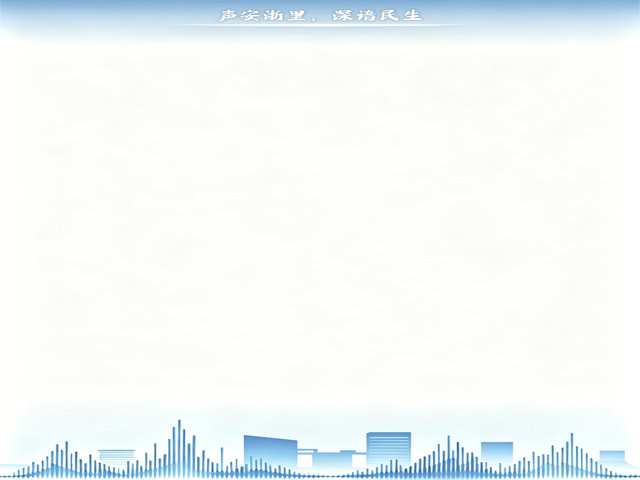
\includegraphics[width=\paperwidth,height=\paperheight]{figures/背景图.jpg}%
}

% 第1页封面图（TikZ 覆盖在背景之上，仅本页）
\thispagestyle{empty}
\begin{tikzpicture}[remember picture, overlay]
  \node[inner sep=0pt] at (current page.center) {%
    
\includegraphics[width=\paperwidth,height=\paperheight]{figures/封面.jpg}%
  };
\end{tikzpicture}
\null
\newpage


%========================================================================================
%	正文
%========================================================================================
%========================================================================================
%	摘要
%========================================================================================
\begin{center}
{\zihao{4}\bfseries 摘\quad 要\par}
\end{center}
\begin{quotation}

\textbf{研究背景与目的：}在城市化持续推进的背景下，噪声污染已成为影响居民生活质量与社会治理成效的重要问题。本报告以浙江省杭州、宁波、温州三地常住居民为调查对象，整合省级年度噪声监测数据、政务投诉文本、问卷与访谈资料，系统分析区域噪声态势、居民感知类型及声环境满意度的形成机制，为噪声精准治理提供实证依据。

\textbf{数据与方法：}首先，对问卷进行有效性筛选与质量检验，获得\textbf{467份有效样本}，样本覆盖不同年龄、文化程度、城市及居住区域，信度与效度检验均满足分析要求。其次，采用\textbf{探索性因子分析}将14项噪声影响题项归纳为身心健康与认知干扰、情绪与社会关系影响、典型环境噪声源干扰、生活场景噪声源干扰四个因子，累积方差解释率为\textbf{64.03\%}，并利用\textbf{KMeans++聚类}识别出五类差异化居民群体。进一步，构建\textbf{有序Logistic回归}并计算决策概率与平均边际效应，同时利用\textbf{结构方程模型}检验噪声影响的传导路径。最后，将有序Logistic与随机森林、XGBoost进行对比，检验可解释模型的预测效果。

\textbf{主要结论：}浙江省2020—2024年环境噪声等效声级呈\textbf{“高位波动、2024年反弹”}特征，杭甬温三市中\textbf{杭州居民的不满意概率相对最高}。噪声感知维度中，\textbf{情绪与社会关系影响对满意度的负向作用最强}，住宅配备隔音墙可使“不满意”概率平均下降\textbf{13.76个百分点}。结构方程模型显示，噪声源既直接降低满意度，又经情绪与社会关系渠道间接影响满意度；模型对比中，有序Logistic在准确率、宏平均F1和Kappa指标上优于随机森林与XGBoost。调研还发现，居民\textbf{官方投诉与法律维权使用率偏低}，\textbf{超过六成居民支持强化噪声治理}，诉求集中于法规标准、排放时段、隔音设施和投诉机制。

\textbf{治理建议：}据此，本报告提出差异化治理建议：首先，针对隔音墙对不满意概率的显著抑制作用，优先推进老旧小区、交通干线和敏感场所的隔音改造；其次，围绕交通、施工等主要噪声源，强化源头降噪、夜间管控与智能监测；最后，针对居民官方投诉率偏低的问题，完善投诉反馈和社区协商机制，并重点关注青少年及身心情绪高敏感群体，为浙江省“浙里宁静”专项行动提供实证支撑。

\vskip1ex
\noindent{\zihao{-4}\heiti 关键词：}~城市噪声污染；探索性因子分析；聚类分析；有序Logistic回归；XGBoost；结构方程模型

\end{quotation}

\clearpage

%========================================================================================
%	目录
%========================================================================================
\setcounter{tocdepth}{2}
\tableofcontents
\clearpage
\listoffigures
\clearpage
\listoftables
\clearpage

\section{项目简介}

\subsection{调查背景}

近年来，环境噪声污染已成为社会关注度高、群众反映强烈的突出民生问题，本研究从不同角度，系统梳理浙江省噪声污染的治理背景与现实痛点，为后续问卷设计与调查范围的确定提供科学依据，也为精准反映杭甬温等核心城市居民的声环境感知奠定基础。

\subsubsection{政策背景：国家与浙江省噪声污染防治政策导向}

噪声污染防治事关民生福祉与生态文明建设，习近平总书记多次强调，要坚持以人民为中心的发展思想，“还自然以宁静、和谐、美丽”，打好污染防治攻坚战，提升生态环境治理现代化水平，这为新时代噪声污染治理工作指明了根本方向。在这一指引下，国家与浙江省先后出台一系列法律法规与政策文件，将噪声污染防治纳入生态文明建设与民生保障的重点工作范畴，也为本次杭甬温三地居民声环境感知调查提供了明确的政策导向、法治依据与现实背景。

《中华人民共和国噪声污染防治法》\scite{ref1}于2022年6月5日正式施行，全面强化\textbf{工业、建筑施工、交通运输、社会生活四大领域}噪声管控，明确政府、企业、公众各方责任，突出源头防控、分类管理、社会共治，着力解决群众关心的施工扰民、商业喧嚣、邻里噪声等现实难题，为全国噪声治理提供了坚实法治保障。

浙江省坚决贯彻国家部署，紧扣高质量发展建设共同富裕示范区目标，持续推进“浙里宁静”建设。先后印发《浙江省噪声污染防治行动计划（2023—2025年）》\scite{ref2}，提出到2025年全省声环境功能区\textbf{夜间达标率达到85\%以上}、噪声投诉明显下降的目标，系统推进制度完善、源头管控、执法监管与数字化治理。2026年3月1日起施行的《浙江省噪声污染防治办法》\scite{ref3}，进一步细化部门监管职责，创新推进宁静小区、宁静工地、宁静公园等创建，将噪声扰民纳入基层社会治理，推动形成齐抓共管格局。

\subsubsection{现实图景：浙江省环境噪声污染问题凸显}

随着浙江省城镇化进程持续推进、城市空间格局不断拓展与城市综合功能日趋完善，人口集聚、交通路网加密、工业生产活跃、商业活动频繁、社区生活多元化等多重因素叠加，交通干线噪声、工业企业生产噪声、建筑施工噪声、广场舞与商业经营等社会生活噪声源的数量、强度与影响范围持续扩大。环境噪声污染已不再是单一的环境问题，而是深度关联城市宜居建设、民生保障与基层社会治理的突出现实难题，长期噪声暴露不仅会损害居民听觉健康、引发焦虑烦躁、睡眠障碍等身心问题，还会降低居民生活满意度与城市归属感，成为制约城市人居环境品质提升、影响群众幸福感与获得感的重要短板。

\fig{图片1.png}{噪声污染影响传导逻辑图}

为系统把握全省声环境质量的变化规律，识别区域噪声污染突出短板，本研究依托浙江省数据开放平台公开监测数据，选取2020—2024年浙江省11个地级市连续五年的城市区域环境噪声、道路交通噪声、声环境功能区定点噪声监测结果，从平均等效连续A声级（LEQ）年度变化、昼夜声环境达标率、不同功能区噪声差异、各地级市空间分布特征以及全省整体变化趋势等多个维度，系统剖析近五年浙江省城市噪声污染现状、区域差异与演变规律，精准识别交通密集区、老旧居住区、工业园区周边等噪声敏感区域的污染特征，为后续开展居民噪声感知调研、梳理治理痛点、提出针对性治理对策提供客观的数据基础与现实依据。

（1）我们按照监测地点的行政区域代码，将三万余份监测数据按地市、年份分组，不对昼夜时间段进行区分，计算得到11个地市各年份的平均等效声级（LEQ），结果热力图如图\ref{fig:heatmap}(a)所示：

（2）为弥补平均等效声级在浙江省噪声污染程度评估时的局限性，本研究根据国家制定的《声环境质量标准（GB3096-2008）》，将监测数据根据时段、区域类型的不同进行达标情况的标注，并对数据按年份、地区进行分类，计算出了11个地级市2020年至2024年的声环境质量达标率，热力图如图\ref{fig:heatmap}(b)所示：

\begin{figure}[H]
\centering
\begin{subfigure}[b]{0.48\textwidth}
  \centering
  
\includegraphics[width=\textwidth]{图片2.png}
  \caption{区域环境噪声等效声级热力图}
\end{subfigure}
\hfill
\begin{subfigure}[b]{0.48\textwidth}
  \centering
  
\includegraphics[width=\textwidth]{图片3.png}
  \caption{声环境质量达标率变化热力图}
\end{subfigure}
\caption{浙江省各地级市噪声等效声级与达标率热力图（2020-2024）}
\label{fig:heatmap}
\end{figure}

从空间分布看，不同城市间噪声压力差异显著，宁波、湖州等城市声级长期处于高位，而浙西南等地区整体声级偏低，区域分化明显；从时间变化看，多数城市的噪声水平呈现阶段性波动特征，\textbf{2023年普遍回落，2024年又出现明显反弹}，反映出噪声治理仍存在反复性与不稳定性。

可见，浙江省各地级市的声环境达标率差异显著：\textbf{杭州市达标率长期处于低位，治理短板突出}；而浙西南等区达标率整体偏高，声环境质量相对稳定。时间上，多数城市的达标率呈现明显的阶段性波动，部分年份达标率出现大幅下滑，反映出噪声治理受外部因素影响较大，常态化管控体系仍需完善。

（3）考虑到噪声暴露在时间维度上并不均衡，本研究进一步将监测数据按上午、下午、晚上、夜间四个时段分别汇总，计算各时段的平均等效声级，并综合全省整体噪声污染情况绘制了双轴组合图，结果如图\ref{fig:temporal}所示：

\begin{figure}[H]
\centering
\begin{subfigure}[b]{0.48\textwidth}
  \centering
  
\includegraphics[width=\textwidth]{env_noise_period.png}
  \caption{不同时段平均等效声级}
\end{subfigure}
\hfill
\begin{subfigure}[b]{0.48\textwidth}
  \centering
  
\includegraphics[width=\textwidth]{env_noise_year.png}
  \caption{平均等效声级与达标率年际变化趋势}
\end{subfigure}
\caption{浙江省不同时段平均等效声级及环境噪声与声环境质量达标率变化趋势（2020-2024）\label{fig:temporal}}
\end{figure}

从时段分布看（图\ref{fig:temporal}(a)），上午、下午、晚上三个时段的平均等效声级较为接近，差异不明显，而夜间时段的平均等效声级显著低于其余三个时段，这与夜间交通流量下降、施工及商业活动基本停止、主要噪声源大幅减少的客观规律一致。需要指出的是，后文居民感知分析显示噪声干扰在夜间最为集中，说明居民对噪声的主观敏感程度并不单纯取决于声级绝对值：夜间背景声级偏低，且与居民休息时段高度重合，\textbf{同等声级造成的干扰反而更强}。因此夜间时段虽在平均声级上并非高值区间，仍需作为声环境管控的重点时段单独考量。

从年际变化看（图\ref{fig:temporal}(b)），全省平均等效声级2020-2022年维持在较高水平，2023年出现明显回落，2024年又快速回升至前期高位，体现出噪声污染防控的阶段性反复；声环境质量达标率则与声级变化呈反向联动关系，随声级的回落与反弹同步波动，说明声级水平仍是影响达标率的核心因素，整体治理成效的持续性有待加强。

\subsubsection{民生诉求：基于噪声投诉文本的痛点挖掘}

相较于宏观的监测数据，民众的真实感受更能反应实际情况。环境治理的成效最终落脚于民众的真实感受。为精准把握噪声污染的民生痛点，本研究利用Python开放环境，通过Scrapy模块和BeautifulSoup解析库，在征求意见以后，对浙江省“民呼我为”政务服务平台2023年至2026年的部分噪音投诉进行了合法定向爬取。随后，再对得到的数据进行Jieba分词处理，加入语气词等停用词进行文本过滤。最后进行词频分析并生成了词云图，直观呈现民生诉求的焦点。

\fig[0.7]{图片5.png}{浙江省噪声投诉词云图}

不难发现，“扰民”是本次分析中的高频词，清晰反映出噪声污染对居民休息、睡眠乃至身心健康的影响，“无法入睡”等表述反映了民众受噪声困扰的强烈不满，为研究提供了民意导向。从噪声来源看，“地铁”“广场舞”“夜间施工”“交通流量大”等词汇高频出现，说明\textbf{交通噪声、社会生活噪声与施工噪声}是民众噪声投诉的主要集中方向。

值得注意的是，\textbf{“投诉无果”“敷衍回复”“无法解决”}这类表述反复出现，折射出部分噪声问题存在治理回应不及时、问题解决不彻底的现实痛点，印证了从民众感知视角开展声环境治理研究的必要性。

\subsection{文献综述与研究缺口}

国内外围绕环境噪声感知与治理已积累较丰富成果。国外研究起步较早，核心结论集中在噪声感知的形成与噪声治理的路径两个方面。就噪声感知而言，居民对环境噪声的感知并非由声级单一决定，而受人口特征、居住环境、社会经济水平乃至个体噪声耐受能力（含神经生理机制）共同影响\scite{ref4}；年龄、性别、职业、文化程度等人口统计学差异均会带来感知偏差，个体耐受能力较弱的人群更易受到噪声侵扰。就噪声治理而言，国外研究侧重源头管控与效益量化，从低噪声路面、限行管控到建筑隔音优化均有涉及，并借助地理空间分析从成本—收益角度评估降噪投入与健康福祉收益\scite{ref5}。但此类结论多以发达国家城市化背景为对象，其噪声类型与治理体制与我国存在差异，相关经验需结合国情本土化适配。

国内研究近年增长较快，已在现状刻画与治理困境两方面形成共识。现状刻画层面，我国城市噪声主要来源于交通、生活与工业三类，区域差异显著，老旧小区与工业园区周边属重点敏感区域，兼具广场舞、动物吠叫等具有本土特色的生活噪声问题。治理困境层面，学者普遍指出政策落实不到位、部门监管边界模糊、责任主体不明、公众参与度不高、治理手段单一等问题，这与潘淑萍提出的监管碎片化、基层治理薄弱、群众取证维权困难等判断一致\scite{ref6}；同时亦关注到传统工业污染治理模式难以应对新型城市噪声的问题\scite{ref7}。

\fig{图片6.png}{噪声污染防治政策体系图}

综观已有研究，仍存在三方面不足。其一，\textbf{数据来源割裂}，客观监测与居民感知多被分开研究，缺乏“监测数据—投诉文本—问卷访谈”三位一体的整合分析；其二，\textbf{机制刻画不足}，感知研究以描述性统计与影响因素识别为主，对声环境满意度“如何形成”的传导路径缺少因果刻画；其三，\textbf{对策缺乏量化支撑}，治理建议趋于同质化，未对隔音设施、投诉响应机制等可干预变量的边际效果进行排序。

据此，本调查以杭州、宁波、温州三市常住居民为对象，整合监测数据、投诉文本与问卷访谈，尝试在数据整合、机制刻画、对策量化三个方面填补上述空白。

\begin{figure}[H]
\centering

\includegraphics[width=\textwidth]{研究局限与本研究创新框架.png}
\caption{研究局限与本研究创新框架}
\label{fig:research_framework}
\end{figure}

\subsection{调查目的}

本次调查旨在聚焦浙江省杭甬温三市居民声环境感知与噪声污染治理需求，系统梳理噪声污染的现实痛点与民众诉求，探究客观监测数据与居民主观体验之间的感知偏差，识别治理薄弱环节，为浙江省优化噪声污染防治策略、推进宁静城市建设提供科学依据与实践参考。

\subsection{调查意义}

\subsubsection{实践意义}

\fig{图片7.png}{噪声治理研究实践意义逻辑图}

本研究立足浙江省噪声污染防治现实需求，以杭州、宁波、温州三大核心城市为实证对象，整合环境监测数据、政务投诉文本与居民问卷调查信息，精准识别交通噪声、社会生活噪声、施工噪声等民生痛点，清晰呈现居民噪声困扰程度、影响时段与治理诉求，为浙江省噪声污染精准防控、靶向治理提供坚实民意支撑与数据参考。研究聚焦\textbf{“监测达标与居民感知脱节”}的现实矛盾，提出\textbf{政府治理、技术应用、公众参与}三维优化路径，有助于推动噪声治理从“数据达标”向“群众满意”转变，切实提升人居环境质量与居民幸福感。同时，本研究形成的主客观结合的噪声评估与治理分析模式，可为浙江省及国内同类城市推进“宁静城市”建设、落实《浙江省噪声污染防治行动计划》提供可复制、可推广的实践范式。

\subsubsection{理论意义}

本研究突破传统噪声污染研究偏重客观监测、忽视主观感知的局限，构建客观数据、主观感知、民生诉求三位一体的城市声环境研究框架，丰富与拓展了环境噪声污染防治领域的理论视角。通过交叉分析、探索性因子分析、有序Logistic回归与SEM结构方程模型等方法，系统揭示不同群体、不同区域噪声感知差异规律与声环境满意度影响机制，深化了城市居民环境感知与主观评价体系的理论认知。本研究将统计建模方法应用于民生导向的环境治理研究，形成标准化实证分析范式，为后续民生视角下的城市环境质量评价、污染治理研究提供理论参考与方法借鉴，助力完善高质量发展建设共同富裕示范区背景下的人居环境理论体系。


\section{调查方案设计}

\subsection{调查对象及范围界定}

\subsubsection{调查对象}

本研究以居民对城市环境噪声污染的主观感知与治理诉求为核心研究内容，将调查对象确定为浙江省杭州、宁波、温州三市常住居民。

本文所指常住居民，为在对应城市连续居住6个月及以上、拥有固定住所、日常主要活动均在本市的人群，涵盖本地户籍人口与外来常住人口。该界定标准排除游客、短期出差人员等临时流动群体，保证调研数据可以真实反映长期身处本地声环境中的居民主观体验。

为提升样本代表性，本次抽样不对受访者的年龄、职业、居住区域进行硬性限定，尽可能覆盖各类人口特征群体。年龄划分五个区间：18岁及以下、19-30岁、31-45岁、46-60岁、61岁及以上；职业包含机关事业单位职工、企业从业者、自由职业者、学生、退休人员等九大类；居住区域分为主城区、城市郊区、县城、乡镇、农村，以此充分区分不同生活场景下居民的噪声暴露差异。

\subsubsection{调查范围}

杭州、宁波、温州三地。

范围选取原因如下：首先，在民意诉求层面，三地在“民呼我为”平台的噪声投诉量占全省比重较高，居民诉求集中，民意反馈具有较强代表性；其次，在监测数据支撑层面，结合全省环境噪声监测数据，杭甬温三市的声环境质量与达标情况更具典型性，与前期现状分析中的典型问题高度契合；最后，在样本典型性层面，作为浙江省经济与人口规模较大的城市，其噪声污染类型多元、矛盾突出，能够为本次研究提供丰富且具有现实参考价值的样本支撑。

\subsection{调查方法}

经过小组讨论与分析，我们最终决定从政策、数据、问卷与访谈三个方面系统开展研究。

\subsubsection{文献调查法}

通过查阅国家及浙江省噪声污染防治相关法律法规、政策文件、统计年鉴与环境监测报告，梳理噪声污染治理的政策导向与现实背景，同时参考国内外声环境感知与噪声治理领域的相关研究成果，为本次调查的整体设计、问卷编制与分析框架提供理论依据与数据支撑。

\subsubsection{问卷调查法}

以杭州、宁波、温州三市常住居民为调查对象，采用线上问卷形式，围绕噪声来源、暴露程度、主观感受、影响评价与治理诉求等维度设计结构化问卷，收集居民对声环境的感知数据。通过统计分析，探究不同人群对噪声污染的感知差异与核心诉求，为后续问题分析与对策建议提供实证依据。

\subsubsection{访谈调查法}

选取部分典型投诉居民与社区工作人员开展半结构化访谈，深入了解噪声污染对居民生活的实际影响、治理过程中的现实困境及公众对噪声治理的意见建议，弥补问卷数据的局限性，挖掘民意反馈背后的深层矛盾，为研究提供更具情境性与深度的质性资料。

\subsection{研究设计}

本次研究框架图如下：

\fig{图片8.png}{研究设计}

\subsubsection{问卷设计}

问卷设计应遵循目的性、逻辑性、明确性、可接受性和效率性等原则，以确保数据收集科学、有效且易于分析。

本文围绕居民对环境噪声的感知、噪声暴露现状、噪声治理评价以及相关认知建议进行设计，在设计上，我们注重问题的逻辑递进与作答便捷性，以确保收集到的数据科学规范、真实有效，为后续的统计分析与问题研判提供坚实支撑。问卷主体共包含五个核心模块：基本信息、噪声暴露与环境感知、噪声治理满意度、噪声治理认知以及噪声治理建议。

\begin{table}[H]
\centering
\caption{问卷具体内容}
\begin{tabular}{M{5cm}M{7cm}}
\bluetoprule
\rowcolor{tabhead}
\thead{模块} & \thead{题项} \\
\hline
\multirow{8}{*}{基本信息} & 性别 \\ \cline{2-2}
 & 年龄 \\ \cline{2-2}
 & 居住地 \\ \cline{2-2}
 & 居住区域类型 \\ \cline{2-2}
 & 职业类型 \\ \cline{2-2}
 & 文化程度 \\ \cline{2-2}
 & 是否为隔音墙 \\ \cline{2-2}
 & 居家办公情况 \\ \hline
\multirow{6}{*}{噪声暴露与环境感知} & 受噪声影响程度 \\ \cline{2-2}
 & 隔音水平评价 \\ \cline{2-2}
 & 各类噪声干扰程度 \\ \cline{2-2}
 & 离噪声源距离 \\ \cline{2-2}
 & 噪音影响时段 \\ \cline{2-2}
 & 噪声负面影响 \\ \hline
\multirow{3}{*}{噪声治理满意度} & 声环境质量满意度 \\ \cline{2-2}
 & 噪声治理满意度 \\ \cline{2-2}
 & 主要应对方式 \\ \hline
\multirow{4}{*}{噪声治理认知} & 投诉渠道认知 \\ \cline{2-2}
 & 国家政策认知 \\ \cline{2-2}
 & 治理必要性认知 \\ \cline{2-2}
 & 责任主体认知 \\ \hline
\multirow{2}{*}{噪声治理建议} & 举措优先度 \\ \cline{2-2}
 & 具体意见 \\
\bluebottomrule
\end{tabular}
\end{table}

\subsubsection{访谈设计}

\textbf{（一）访谈对象}

本次访谈聚焦两类典型噪声易感群体，选取杭州、宁波、温州三地主城区老旧小区独居老人、郊区工厂周边一线职工作为访谈对象。

老旧小区独居老人与工厂一线职工，分别代表城市生活区与工业区的典型噪声敏感人群。前者居住环境隔音薄弱、对噪声高度敏感，后者长期暴露于工业、交通及施工噪声中，两类群体均能精准反映杭甬温三地噪声污染的民生痛点，具备高度代表性。

\textbf{（二）访谈内容}

对象一为主城区老旧小区独居老人，提纲如下：

\begin{enumerate}[label=（\arabic*）,leftmargin=2.5em,itemsep=0.5ex]
\item 您在此处居住多久？房屋墙体隔音效果如何？
\item 日常生活中受到哪些环境噪声影响，影响程度如何？
\item 邻居生活噪声、广场舞、犬吠声等是否对您造成干扰？
\item 您居住区域整体隔音水平如何？哪个时段噪声影响最大？
\item 噪声是否影响您的睡眠、精神状态，有无耳鸣、烦躁等不适？
\item 您对居住地声环境质量、本地噪声治理工作是否满意？
\item 您是否了解12345、浙里办等噪声投诉渠道，是否听说过《中华人民共和国噪声污染防治法》？
\item 您认为是否需要强化浙江省噪声治理？噪声治理的责任主体是谁？
\item 针对改善噪声污染，您有哪些具体意见与建议？
\end{enumerate}

对象二为郊区工厂周边一线职工，提纲如下：

\begin{enumerate}[label=（\arabic*）,leftmargin=2.5em,itemsep=0.5ex]
\item 您在此职工宿舍居住多久？墙体隔音条件如何？是否需要居家办公？
\item 日常生活中受噪声影响程度如何，哪种噪声干扰最为严重？
\item 装修施工、商业经营、公共活动类噪声是否对您产生干扰？区域隔音水平怎么样？
\item 距离噪声源远近如何？哪个时段噪声影响最大？
\item 噪声是否造成睡眠障碍、精神疲惫、注意力下降等问题？
\item 长期噪声环境是否引发耳鸣、心悸、头晕等身体不适？
\item 遭遇噪声扰民时，您及同事主要采取哪些应对方式？
\item 您是否了解12345、浙里办等投诉渠道，是否知晓《中华人民共和国噪声污染防治法》？
\item 您认为是否需要强化浙江省噪声治理？责任主体包含哪些？
\item 针对工厂周边噪声污染治理，您有哪些具体的意见与建议？
\end{enumerate}

\subsection{样本容量确定}

样本容量的科学确定是保障问卷调查数据可靠性、统计分析有效性的核心前提，直接影响后续实证研究结果稳定性与准确性。以下是确定样本容量的方法。

\subsubsection{问卷预发放}

为确保正式问卷的可靠性，本研究先抽取杭甬温居民通过预调查的方式先发放了108份电子问卷，以作答时间少于60秒作为无效问卷的判定标准，经初步筛选后得到有效问卷99份，则问卷有效率约为92\%。该结果为后续正式调查的样本量修正提供了现实依据，也验证了问卷整体作答体验良好，题项设置基本合理。具体情况如下：

\begin{table}[H]
\centering
\caption{问卷预调研回收情况}
\label{tab:presurvey}
\rowcolors{2}{tablight}{white}
\begin{tabular}{M{3.5cm}M{3.5cm}M{3.5cm}M{3.5cm}}
\bluetoprule
\rowcolor{tabhead}
\thead{入样城市} & \thead{实发问卷} & \thead{有效问卷} & \thead{有效率} \\
\hline
杭州市 & 32 & 30 & 93.8\% \\
宁波市 & 46 & 42 & 91.3\% \\
温州市 & 30 & 27 & 90.0\% \\
合计 & 108 & 99 & 91.7\% \\
\bluebottomrule
\end{tabular}
\end{table}

\subsubsection{计算样本容量}

本研究采用简单随机抽样下的总体比例估计法确定最小样本量，计算公式为：

\begin{equation}
n_0=\frac{z_{\alpha/2}^{2}\cdot p(1-p)}{e^{2}}
\end{equation}

其中 $z_{\alpha/2}$ 为95\%置信水平下对应的标准正态分布分位数，取值1.96，$p$ 表示总体比例最保守情况的估计值，取值0.5，$e$ 为允许抽样的边际误差，为了提高结果的精度，我们设定为0.05。代入公式我们得到初始样本量：

\begin{equation}
n_1=\frac{1.96^{2}\times0.5\times0.5}{0.05^{2}}\approx384
\end{equation}

本研究的调查对象为杭州、宁波、温州三市常住居民，根据最新人口统计数据，三市常住居民总数约为 $N=3230.9$ 万，由于采用有限总体抽样，需对初始样本量进行有限总体修正，修正公式为：

\begin{equation}
n_2=n_1\times\frac{N}{N+n_1-1}\approx384
\end{equation}

由于三市常住居民总数 $N$ 远大于初始样本量 $n_1$，因此修正后仍取原来的数目。本研究采用分区域随机抽样，问卷设计效益（deff）设为1.1，继续修正为：

\begin{equation}
n_3=n_2\times\mathrm{deff}\approx422.4
\end{equation}

基于预调查得到的问卷有效率为 $r=92\%$，对样本量进行最终修正，得到正式调查所需发放的问卷总数，公式为：

\begin{equation}
n_4=\frac{n_3}{r}=\frac{422.4}{0.92}\approx459
\end{equation}

为了进一步保证数据有效性，以及考虑到现实需求，我们最终决定发放问卷480份，具体各市问卷情况如表\ref{tab:presurvey}所示。

\subsection{问卷回收情况}

问卷发放周期为2026年7月9日至2026年7月25日，共发放问卷520份，回收问卷493份，问卷回收率为94.81\%。对回收问卷进行有效性筛选，剔除作答时长不足100秒、所有题项选择同一答案、量表题项存在明显作答矛盾的无效问卷后，最终得到有效问卷467份（具体如表\ref{tab:recovery}）。

有效样本中，男性260人，女性207人；年龄分布以18-35岁群体为主，占比61.24\%；文化程度以本科及以上学历为主，占比73.02\%；样本在居住城市、居住区域类型、职业状态等维度分布均衡，具有良好的代表性，可用于后续统计分析。

\begin{table}[H]
\centering
\caption{问卷最终回收情况}
\label{tab:recovery}
\rowcolors{2}{tablight}{white}
\begin{tabular}{M{3.5cm}M{3.5cm}M{3.5cm}M{3.5cm}}
\bluetoprule
\rowcolor{tabhead}
\thead{入样城市} & \thead{回收问卷} & \thead{有效问卷} & \thead{有效率} \\
\hline
杭州市 & 142 & 132 & 93.0\% \\
宁波市 & 203 & 192 & 94.6\% \\
温州市 & 148 & 143 & 96.6\% \\
合计 & 493 & 467 & 94.7\% \\
\bluebottomrule
\end{tabular}
\end{table}

\subsection{问卷误差分析}

本次针对杭甬温三地居民开展环境噪声感知问卷调查，在数据收集、整理过程中不可避免存在误差，为保障研究结果的准确性与可靠性，对两类误差来源进行系统分析，并制定对应控制措施。

\subsubsection{抽样误差}

抽样误差是因采用抽样调查而非全面普查，样本结构与总体真实情况存在偏差所产生的随机误差，属于不可避免的统计性误差。

本次调查通过线上发放电子问卷开展，选取杭州、宁波、温州各类典型居住区域的不同人群作为调查样本。受样本覆盖范围限制，样本在年龄、职业、居住区域、居住年限等维度的分布，无法完全匹配区域全体居民的真实结构；同时受样本量限制，部分小众群体的噪声感知特征未能得到充分体现，进而导致样本统计结果与总体真实水平存在小幅偏差。这类误差可以通过合理扩大样本量、优化抽样结构降低，但无法完全消除。

\subsubsection{非抽样误差}

非抽样误差是由人为因素引发的系统性偏差，对本次调研数据质量的影响较为突出。

其来源主要集中在实际作答与数据处理两个阶段：在实际作答环节，部分受访者存在敷衍心态，表现为填写时长过短、答案逻辑矛盾或量表选项单一重复等规律性作答行为，导致问卷有效性不足；同时，由于部分受访者对噪声相关概念认知模糊，常依靠主观感受随意作答，进一步造成了数据的客观失真。而在数据回收、筛选与录入阶段，无效问卷的误留存以及人工录入过程中的操作失误，也共同构成了本次调研的非抽样误差来源。

\subsubsection{误差控制}

为有效控制两类误差对研究结论的干扰，本研究从抽样、作答到数据处理的全流程实施了较为系统的误差控制措施。

\textbf{（1）在调查设计层面}，参考同类环境感知问卷的成熟量表，结合预调查反馈优化题项表述，降低理解歧义，采用分层抽样设计以降低抽样误差，合理控制问卷长度，避免受访者因疲劳产生系统性偏差。

\textbf{（2）在数据收集层面}，同步通过线上、线下渠道采集样本，覆盖不同数字化能力群体，在问卷中穿插陷门题与方向反转题，识别并剔除随意作答的无效问卷，实时监控各城市样本采集进度，动态调整数据收集策略。

\textbf{（3）在数据后处理层面}，比对样本分布与总体人口学特征，按需采用事后分层加权修正样本偏差，运用多重插补法处理可控缺失变量，对存在系统性缺失的变量进行审慎处置，全部统计分析均依托清洗核验后的高质量数据开展。通过以上分层管控手段，本研究有效保障调查数据的信度与效度，为后续描述性统计、组间差异检验、回归建模等定量分析工作奠定可靠数据基础。


\section{数据预处理}

\subsection{数据清洗}

在问卷收集完成并汇总后，首先对问卷进行系统性审核，剔除无效问卷，仅保留有效样本开展后续分析，以保障数据质量与研究有效性。无效问卷的剔除标准如下：

\textbf{（1）}纸质问卷中，字迹模糊、问卷有效内容破损，导致无法提取有效信息的问卷，视为无效问卷并剔除。

\textbf{（2）}电子问卷中，答题总时长不超过50秒的问卷，视为无效问卷并剔除。

\textbf{（3）}所有问卷中，出现连续3题及以上未作答、答案与问题无关、答案数量与题目要求不一致、答卷中大部分内容选择同一选项，或出现明显规律性作答痕迹的问卷，均视为无效问卷并剔除。

\subsection{缺失值处理}

对于清洗后有效问卷中仍存在的缺失值，本研究采用如下处理方式：

首先对缺失率超过10\%的变量进行评估，主要是“居家办公情况”一题，约有36.62\%的受访者为学生、退休人员或无业待业者，缺失比例较高（如图\ref{fig:homeoffice}），将不进行插补，并在描述性统计中单独进行分析。除此之外，对于“不清楚居所是否为隔音墙”选项，将其与“无隔音墙”合并为一类处理，后续分析中不再单独区分。

对于缺失率低于10\%的变量，分类变量采用该变量的众数进行填充，连续变量（如量表题）采用均值或中位数进行填充，以在不显著影响样本量的前提下，降低缺失值对后续统计分析的干扰。

\fig{图片9.png}{居家办公题项缺失情况\label{fig:homeoffice}}

\subsection{数据编码}

为实现问卷数据的标准化处理与后续量化分析，本研究对回收后的有效问卷进行统一的数据编码处理，将问卷中各类文字、选项信息转化为可用于统计分析的数字代码。

针对性别、年龄、居住地、职业、文化程度等人口统计学类单选题，按照选项顺序依次赋予对应数字编码实现量化转换。对于受噪声影响程度、隔音水平评价、治理满意度等李克特五级量表类题目，将程度表述依次赋值为1-5分，统一量化标准以便开展均值、方差及相关性分析。针对多选类题目，采用二分法编码形式，将受访者选择的选项标记为1，未选择项标记为0，精准区分不同噪声类型、应对方式等的选择差异。针对开放题与访谈文本内容，采用质性编码方式，围绕噪声干扰类型、健康影响、治理诉求、政策认知等核心主题进行概念提炼，归纳形成核心范畴，将文字性访谈资料转化为可分析的定性数据。具体如下表：

\begin{table}[H]
\centering
\caption{问卷编码规则}
\resetrowcolors
\begin{tabular}{M{2.4cm}M{3.4cm}M{2.4cm}p{5.6cm}}
\bluetoprule
\rowcolor{tabhead}
\thead{变量分类} & \thead{变量名称} & \thead{变量类型} & \multicolumn{1}{c}{\thead{编码规则}} \\
\hline
\multirow{8}{*}{基本信息} & 性别 & 二分类变量 & 1=男，2=女 \\ \cline{2-4}
 & 年龄 & 有序分类变量 & 1=第一个选项，2=第二个选项，以此类推 \\ \cline{2-4}
 & 居住地 & 无序分类变量 & 1=第一个选项，2=第二个选项，以此类推 \\ \cline{2-4}
 & 居住区域类型 & 无序分类变量 & 1=第一个选项，2=第二个选项，以此类推 \\ \cline{2-4}
 & 职业类型 & 无序分类变量 & 1=第一个选项，2=第二个选项，以此类推 \\ \cline{2-4}
 & 文化程度 & 有序分类变量 & 1=第一个选项，2=第二个选项，以此类推 \\ \cline{2-4}
 & 是否为隔音墙 & 无序分类变量 & 1=第一个选项，2=第二个选项，以此类推 \\ \cline{2-4}
 & 居家办公情况 & 有序分类变量 & 1=第一个选项，2=第二个选项，以此类推 \\ \hline
\multirow{6}{*}{噪声暴露与环境感知} & 受噪声影响程度 & 李克特5级量表 & 1=影响非常大，5=几乎没有影响 \\ \cline{2-4}
 & 隔音水平评价 & 李克特5级量表 & 1=很好，5=很差 \\ \cline{2-4}
 & 各类噪声干扰程度 & 李克特5级量表 & 1=无干扰，5=严重干扰 \\ \cline{2-4}
 & 离噪声源距离 & 有序分类变量 & 1=第一个选项，2=第二个选项，以此类推 \\ \cline{2-4}
 & 噪音影响时段 & 有序分类变量 & 1=第一个选项，2=第二个选项，以此类推 \\ \cline{2-4}
 & 噪声负面影响 & 李克特5级量表 & 1=不认同，5=认同 \\ \hline
\multirow{3}{*}{噪声治理满意度} & 声环境质量满意度 & 李克特5级量表 & 1=非常不满意，5=非常满意 \\ \cline{2-4}
 & 噪声治理满意度 & 李克特5级量表 & 1=非常不满意，5=非常满意 \\ \cline{2-4}
 & 主要应对方式 & 多重响应变量 & 采用二进制编码，被选择编码为1，未选择编码为0 \\ \hline
\multirow{4}{*}{噪声治理认知} & 投诉渠道认知 & 李克特5级量表 & 1=非常不了解，5=非常了解 \\ \cline{2-4}
 & 国家政策认知 & 李克特5级量表 & 1=非常不了解，5=非常了解 \\ \cline{2-4}
 & 治理必要性认知 & 李克特5级量表 & 1=完全没有必要，5=非常有必要 \\ \cline{2-4}
 & 责任主体认知 & 多重响应变量 & 采用二进制编码，被选择编码为1，未选择编码为0 \\ \hline
\multirow{2}{*}{噪声治理建议} & 举措优先度 & 多重响应变量 & 采用二进制编码，被选择编码为1，未选择编码为0 \\ \cline{2-4}
 & 具体意见 & 无结构文本数据 & 开放式编码 \\
\bluebottomrule
\end{tabular}
\end{table}


\section{问卷质量分析}\label{sec:quality}

\subsection{随机性检验}

为检验样本是否存在抽样偏差，本研究采用\textbf{游程检验}，利用SPSS对性别、年龄、现居住地、现居住区域、职业类型、文化程度6项人口统计学变量进行分析。该检验通过比较实际游程数与随机条件下的期望游程数，判断样本在采集顺序上的随机程度；检验值按各变量的中位数设定（性别取切分值2），有效样本为467份，结果如表\ref{tab:runs}所示。
\begin{table}[H]
\centering
\caption{游程检验结果}
\label{tab:runs}
\rowcolors{2}{tablight}{white}
\begin{tabular}{M{2.8cm}M{1.6cm}M{1.6cm}M{1.6cm}M{1.6cm}M{1.6cm}M{1.6cm}}
\bluetoprule
\rowcolor{tabhead}
\thead{参数} & \thead{性别} & \thead{年龄} & \thead{现居住地} & \thead{现居住区域} & \thead{职业类型} & \thead{文化程度} \\
\hline
检验值 & 2 & 3 & 2 & 2 & 4 & 4 \\
个案数$<$检验值 & 260 & 167 & 132 & 134 & 196 & 195 \\
个案数$\ge$检验值 & 207 & 300 & 335 & 333 & 271 & 272 \\
总个案数 & 467 & 467 & 467 & 467 & 467 & 467 \\
游程数 & 177 & 174 & 157 & 164 & 204 & 197 \\
$Z$ & -5.115 & -4.191 & -3.815 & -3.183 & -2.328 & -2.967 \\
渐近显著性(双尾) & $<0.001$ & $<0.001$ & $<0.001$ & 0.001 & 0.020 & 0.003 \\
\bluebottomrule
\end{tabular}
\end{table}

检验结果显示，6项变量的显著性均小于0.05，说明样本在采集顺序上并非完全随机。其中，性别、年龄和现居住地的显著性均小于0.001，职业类型的显著性最高但也仅为0.020，表明各变量均存在不同程度的系统性排列。该现象主要与问卷按城市分批发放和回收有关，同一城市样本在数据序列中相对集中；其反映的是数据采集顺序特征，并不影响样本的覆盖范围与代表性，数据仍可用于后续分析。

\subsection{相关性分析}

由于“受噪声影响程度”采用反向计分，分析前先进行正向化处理；考虑到相关变量多为有序变量，本研究采用\textbf{Spearman秩相关分析}，利用SPSS对467份有效样本进行检验，以识别居民整体噪声感知与各类噪声源、噪声负面影响之间的关联，结果如图\ref{fig:spearman}所示。

\fig[0.98]{spearman_correlation.png}{居民整体噪声感知与各题项的Spearman相关分析结果\label{fig:spearman}}

结果显示，各题项与整体噪声感知\textbf{均呈显著正相关}（$P<0.05$），多数达到$P<0.001$水平。其中，交通噪声影响、公共活动噪声影响和装修/施工噪声影响的关联较强，是影响整体声环境体验的主要噪声源；其余题项多为弱相关，但显著性均满足要求。整体而言，各类噪声干扰越强，居民的睡眠、注意力、情绪和身心健康所受负面影响越明显。

\subsection{信度分析}

为检验问卷量表的可靠性与内部一致性，本研究采用\textbf{克朗巴哈系数（Cronbach's Alpha）}对22个量表题项进行信度分析（含14个噪声影响题项与受噪声影响程度、隔音水平评价、离噪声源距离、两项满意度评价及三项治理认知等8个其他量表题项）。其中“受噪声影响程度”为\textbf{反向计分}题（1=影响非常大，5=几乎没有影响），计算前已作正向化处理，结果如下表。

\begin{table}[H]
\centering
\caption{信度分析结果}
\rowcolors{2}{tablight}{white}
\begin{tabular}{M{8cm}M{5cm}}
\bluetoprule
\rowcolor{tabhead}
\thead{指标} & \thead{数值} \\
\hline
克隆巴赫Alpha & 0.735 \\
项数 & 22 \\
\bluebottomrule
\end{tabular}
\end{table}

结果显示，克隆巴赫Alpha为0.735，表明问卷量表具有可接受的信度。

\subsection{效度检验}

为检验量表题项的结构效度，本研究采用\textbf{KMO取样适切性量数}和\textbf{巴特利特球形检验}，利用SPSS对参与后续因子分析的14个噪声影响题项进行分析，结果如下表。

\begin{table}[H]
\centering
\caption{效度检验结果}
\rowcolors{2}{tablight}{white}
\begin{tabular}{M{8cm}M{5cm}}
\bluetoprule
\rowcolor{tabhead}
\thead{指标} & \thead{数值} \\
\hline
KMO取样适切性量数 & 0.815 \\
巴特利特球形检验近似卡方 & 2119.289 \\
自由度 & 91 \\
显著性 & $<0.001$ \\
\bluebottomrule
\end{tabular}
\end{table}

结果显示，KMO值为0.815，巴特利特球形检验显著性小于0.001，表明量表适合进行因子分析，结构效度较好。

\section{描述性统计分析}

基于本次杭甬温三市环境噪声感知调研的467份有效问卷数据，本次调研从受访者样本特征、噪声暴露与感知整体情况、声环境认知现状等维度开展全面的描述性统计分析，系统呈现调研样本的结构特征、居民噪声暴露与感知的整体态势，以及对声环境治理的认知与需求情况。

\subsection{受访者样本特征分析}

\subsubsection{人口统计学特征}

\begin{figure}[H]
\centering
\begin{subfigure}[b]{0.46\textwidth}
  \centering
  
\includegraphics[width=\textwidth]{板块1_性别构成.png}
  \caption{性别构成}
\end{subfigure}
\hfill
\begin{subfigure}[b]{0.46\textwidth}
  \centering
  
\includegraphics[width=\textwidth]{板块2_城市分布.png}
  \caption{城市分布}
\end{subfigure}

\vspace{0.6em}

\begin{subfigure}[b]{0.46\textwidth}
  \centering
  
\includegraphics[width=\textwidth]{板块3_年龄构成.png}
  \caption{年龄构成}
\end{subfigure}
\hfill
\begin{subfigure}[b]{0.46\textwidth}
  \centering
  
\includegraphics[width=\textwidth]{板块4_文化程度.png}
  \caption{文化程度}
\end{subfigure}

\vspace{0.6em}

\begin{subfigure}[b]{0.46\textwidth}
  \centering
  
\includegraphics[width=\textwidth]{板块5_居住区域.png}
  \caption{居住区域}
\end{subfigure}
\hfill
\begin{subfigure}[b]{0.46\textwidth}
  \centering
  
\includegraphics[width=\textwidth]{板块6_职业构成.png}
  \caption{职业构成}
\end{subfigure}
\caption{受访者样本人口统计学特征\label{fig:profile}}
\end{figure}

\textbf{（1）性别与年龄特征}

如图\ref{fig:profile}(a)、(c)所示，样本中男性260人（55.67\%），女性207人（44.33\%），男性比例略高于女性。年龄结构以中青年为主体，31-45岁群体比例最高（31.69\%），19-30岁（27.41\%）及46-60岁（22.70\%）次之，18岁以下（8.35\%）及61岁及以上（9.85\%）比例相对较低。

\textbf{（2）城市与居住区域分布}

如图\ref{fig:profile}(b)、(e)所示，样本数据采集自杭州、宁波、温州三市，分布与前期调研权重设计一致。其中宁波市样本量最大（192人，41.11\%），温州市（143人，30.62\%）与杭州市（132人，28.27\%）次之。居住区域类型方面，城市主城区（134人，28.69\%）与城市郊区（132人，28.27\%）占比相近，县城（90人，19.27\%）、乡镇（74人，15.85\%）与农村（37人，7.92\%）依次递减，样本以城区居民为主，同时保留了相当比例的乡镇与农村样本。

\textbf{（3）受教育程度}

如图\ref{fig:profile}(d)所示，样本中本科及以上学历者合计超过四成，其中本科学历160人（34.26\%），硕士及以上31人（6.64\%）。此外，高中/中专/技校（19.27\%）、大专（17.34\%）、初中（14.56\%）、小学及以下（7.92\%）等不同学历层次均有覆盖。

\textbf{（4）职业分布}

如图\ref{fig:profile}(f)所示，样本职业类型较为多元。企业工作人员比例最高（130人，27.84\%），学生群体次之（119人，25.48\%）。自由职业者/个体工商户（65人，13.92\%）、农林牧渔从业者（38人，8.14\%）等亦占有一定比例，基本覆盖了城市主要就业群体。

\subsubsection{生活状态特征}

\fig{图片11.png}{隔音墙状态}

居住隔音配套是决定居民噪声暴露水平的关键客观硬件条件，本次调研专门设置住宅隔音墙相关题项统计现状。数据显示仅28\%受访者家中配备专业隔音墙体或隔音门窗配套，高达72\%的住宅无隔音设施或受访者无法确认房屋隔音配置。住宅隔音设施配套失衡是老旧小区改造遗留的共性短板，新建商品房隔音门窗普及率更高，而建成10年以上老旧楼栋几乎无专业隔音构造，这一硬件差距造成居民日常噪声暴露强度分层，也与老旧小区占比偏高的特征形成互证。老旧小区墙体单薄、窗户密封性差，导致外部交通、施工噪声可直接穿透进入室内，大幅加剧居民主观困扰程度，也是后续治理需要重点补齐的硬件短板。

\subsection{噪声暴露与感知整体情况}

\fig{图片12.png}{噪声暴露全景分析}

\subsubsection{噪声困扰程度分布}

本研究通过李克特5级量表对噪声影响程度进行评估。

结果显示：认为噪声“影响一般”与“影响较大”的受访者占比并列最高，均为30.62\%；其次为“偶尔有影响”（22.70\%）、“几乎没有影响”（11.35\%）和“影响非常大”（4.71\%）。超60\%的受访者认为噪声对生活存在中等及以上影响，其中超三成居民受到较大程度干扰，反映出杭甬温三市居民的噪声困扰问题较为普遍，噪声污染已成为影响居民生活质量的重要环境问题。

\subsubsection{各类噪声源干扰特征}

从干扰程度排序来看，交通噪声（3.09分）与施工噪声（3.01分）的干扰强度最高，二者得分均超过3分，处于中等偏上水平；其后依次为动物噪声（2.95分）、公共活动噪声（2.83分）、生活噪声（2.76分）与商业噪声（2.70分）。整体而言，交通噪声与施工噪声是杭甬温三市居民面临的最主要噪声干扰源，这与城市交通流量大、工程建设活动频繁的发展特征高度契合。

\subsubsection{噪声影响时段与距离特征}

从时段特征来看，噪声影响呈现明显的夜间集中倾向，晚上和深夜受到噪声干扰的受访者数量最多，分别为138人和135人，白昼人数占比较少。这一分布特征表明，夜间噪声对居民的影响更为突出，与居民休息、睡眠的核心时段高度重合，更容易对生活质量造成负面影响。

从声源距离分布来看，认为噪声源距离适中的人数最多，对应161人；其次为距离较近（102人）和较远（101人）；近在咫尺（36人）和非常远（67人）的受访者占比相对较低。这一结果说明，大部分居民面临的噪声源来自周边50米范围内的环境，以社区及周边活动、道路交通等近距离声源为主，这类噪声更易对居民生活产生持续且直接的干扰。

整体来看，噪声影响的时空特征与居民的生活作息和居住环境高度相关，夜间与近距离噪声是当前治理工作中需要重点关注的方向。

\subsection{声环境认知现状}

\fig{图片13.png}{满意度总览}

\subsubsection{声环境与治理满意度评价}

对于声环境质量满意度，超44\%的受访者对当前的声环境质量持不满意态度，仅约27\%的受访者持满意态度，反映出杭甬温三市居民对当前声环境质量的整体评价偏低，声环境质量与居民的预期仍存在较大差距。

对于噪声治理工作满意度，约40\%的受访者对当前的噪声治理工作持满意态度，超30\%的受访者持一般态度，仅约30\%的受访者持不满意态度，居民对噪声治理工作的满意度显著高于对声环境质量的满意度，反映出居民对本地噪声治理工作的努力有一定的认可，但治理成效仍未达到居民的预期，有较大的提升空间。现有管控力度、覆盖范围、整改处置效率尚未完全消解长期噪声侵扰带来的负面体验，治理成效存在明显滞后性，管控行动转化为实际环境仍存在堵点。

\subsubsection{居民应对方式分析}

\fig{图片14.png}{面对噪声的应对方式}

整体来看，居民遭遇噪声污染时，最倾向于采用自主协商、向社区/物业反馈的私力救济与基层救济方式，同时自我防护也是重要的应对手段。而官方渠道投诉、法律途径维权等公力救济方式的采用比例相对较低，仅约40\%的受访者会选择官方投诉渠道，不足20\%的受访者会采取法律途径维权，反映出当前居民的噪声维权渠道的使用意愿仍有较大的提升空间，维权渠道的便捷性、有效性仍需进一步优化。

\subsubsection{噪声治理认知与需求}

\fig{图片15.png}{噪声治理倾向\label{fig:tendency}}

由图\ref{fig:tendency}可知，超61\%的受访者认为强化浙江省环境噪声治理有必要或非常有必要，仅约18\%的受访者认为没有必要或完全没有必要。这说明绝大多数居民对噪声治理的必要性有高度的认知，具备较强的噪声治理意愿与需求，为噪声治理工作的推进提供了良好的群众基础。

\fig{图片16.png}{噪声治理需求\label{fig:demand}}

由图\ref{fig:demand}可知，居民对噪声治理的需求呈现出“制度完善优先、源头管控核心、硬件保障配套、监管执法兜底”的特征，最核心的需求是完善噪声管控的法律法规与标准，体现现有管控细则仍存在模糊地带，基层执法缺少清晰量化分贝、时限依据。

其次居民对施工、交通噪声的时段管控、隔音硬件设施建设、投诉处理机制优化等方面也有强烈的需求，群众更期待兼顾制度完善与实体降噪工程同步推进，这为后续噪声治理工作的方向与重点提供了清晰的民意依据。


\section{噪声影响维度的探索性因子分析降维}

噪声影响的14个题项之间存在较强相关性，若直接纳入后续模型会带来解释上的冗余。为提取结构清晰的潜在维度，本研究对上述题项进行探索性因子分析，将分散的题项信息压缩为少数几个相互独立的公因子，并为后续聚类分析与回归建模提供输入变量。

\subsection{适用性检验}

因子分析的前提是题项之间存在足够的\textbf{共同变异}。第四章的效度检验已针对这14个噪声影响题项完成KMO取样适切性检验与巴特利特球形检验，得到KMO取样适切性量数为0.815，巴特利特球形检验近似卡方值为2119.289（$df=91$，$p<0.001$）；信度检验得到总量表克隆巴赫Alpha系数为0.735。KMO值处于良好水平，球形检验拒绝了变量相互独立的原假设，说明题项间相关性显著、内部一致性良好，满足因子分析的前提条件，故此处不再重复报告检验细节。

\subsection{噪声影响的四维因子解构}

本研究以\textbf{主成分分析法}提取公因子，并采用凯撒正态化最大方差法进行旋转。旋转的目的是重新分配各因子所解释的方差，使因子载荷向0或1两极分化，从而让每个题项尽可能只在一个因子上呈现高载荷，便于因子命名与解释。

\subsubsection{公因子方差}

\begin{table}[H]
\centering
\caption{公因子方差}
\label{tab:communality}
\rowcolors{2}{tablight}{white}
\begin{tabular}{M{6cm}M{2.5cm}M{2.5cm}M{3cm}}
\bluetoprule
\rowcolor{tabhead}
\thead{题项} & \thead{初始值} & \thead{提取值} & \thead{提取程度} \\
\hline
交通噪声影响 & 1 & 0.539 & 中 \\
周围人生活噪声影响 & 1 & 0.501 & 中 \\
装修/施工噪声影响 & 1 & 0.750 & 高 \\
商业经营噪声影响 & 1 & 0.648 & 较高 \\
公共活动噪声影响 & 1 & 0.611 & 较高 \\
动物噪声影响 & 1 & 0.634 & 较高 \\
噪声入睡情况影响 & 1 & 0.616 & 较高 \\
噪声中断睡眠影响 & 1 & 0.572 & 中 \\
噪声注意力影响 & 1 & 0.742 & 高 \\
噪声身边关系影响 & 1 & 0.655 & 较高 \\
噪声精神状态影响 & 1 & 0.757 & 高 \\
噪声对身体健康影响 & 1 & 0.690 & 较高 \\
噪声对听觉影响 & 1 & 0.580 & 中 \\
噪声对极端情绪影响 & 1 & 0.668 & 较高 \\
\bluebottomrule
\end{tabular}
\end{table}

表\ref{tab:communality}给出各题项的公因子方差。初始值均为1，代表每个题项所包含的全部信息量；提取值表示公因子对该题项信息的解释比例，数值越大说明该题项的信息被公因子保留得越充分。结果显示，全部题项的提取值均大于0.5，处于中等及以上水平，其中“装修/施工噪声影响”“噪声精神状态影响”“噪声注意力影响”的提取值分别为0.750、0.757、0.742，提取程度为“高”；其余题项提取值介于0.501$\sim$0.690之间，提取程度为“中”或“较高”。所有题项的信息都能被公因子有效解释，无信息损失严重的题项，无需删除处理。

\begin{table}[H]
\centering
\caption{总方差解释}
\label{tab:variance}
\begin{subtable}[t]{0.49\textwidth}
\centering
\caption{提取载荷平方和}
\small
\setlength{\tabcolsep}{3pt}
\rowcolors{2}{tablight}{white}
\begin{tabular}{M{1.2cm}M{2.1cm}M{1.7cm}M{1.7cm}}
\bluetoprule
\rowcolor{tabhead}
\thead{成分} & \thead{可解释信息量} & \thead{方差百分比} & \thead{向上累积\%} \\
\hline
因子1 & 4.230 & 30.22\% & 30.22\% \\
因子2 & 1.950 & 13.93\% & 44.14\% \\
因子3 & 1.678 & 11.99\% & 56.13\% \\
因子4 & 1.105 & 7.89\% & 64.03\% \\
\bluebottomrule
\end{tabular}
\end{subtable}
\hfill
\begin{subtable}[t]{0.49\textwidth}
\centering
\caption{旋转载荷平方和}
\small
\setlength{\tabcolsep}{3pt}
\rowcolors{2}{tablight}{white}
\begin{tabular}{M{1.2cm}M{2.1cm}M{1.7cm}M{1.7cm}}
\bluetoprule
\rowcolor{tabhead}
\thead{成分} & \thead{可解释信息量} & \thead{方差百分比} & \thead{向上累积\%} \\
\hline
因子1 & 2.735 & 19.53\% & 19.53\% \\
因子2 & 2.622 & 18.73\% & 38.26\% \\
因子3 & 1.824 & 13.03\% & 51.29\% \\
因子4 & 1.783 & 12.73\% & 64.03\% \\
\bluebottomrule
\end{tabular}
\end{subtable}
\end{table}

表\ref{tab:variance}报告了公因子对原始信息的解释能力。旋转前，第一个因子单独解释了30.22\%的方差，旋转后其贡献率回落至19.53\%，而四个因子的方差贡献率分别为19.53\%、18.73\%、13.03\%和12.73\%，分布趋于均衡，说明旋转有效削弱了单一因子的主导地位。四个公因子的累积方差解释率为\textbf{64.03\%}，即原有14个题项六成以上的信息可由这四个因子承载，降维效果良好。

\subsubsection{公因子提取与命名}

\fig{图片17.png}{因子分析碎石图\label{fig:scree}}

公因子的提取数量结合碎石图拐点与特征值大小共同判定。碎石图以因子序号为横轴、对应特征值为纵轴，其中特征值代表单一公因子能够承载的原始变量信息量，其衰减规律可直观反映各因子的解释力度。

如图\ref{fig:scree}所示，折线在前4个因子区间内下降陡峭，自第5个因子起斜率大幅收窄、走势趋于平缓，曲线贴近横轴缓慢延伸，在第4、5因子之间形成明显的“肘部拐点”。数值上，前4个因子的特征值分别为4.230、1.950、1.678和1.105，均大于1；第5个因子特征值降至0.777，已低于1的临界阈值。碎石图拐点与特征值大于1准则的判定结果一致，不存在判定冲突，故提取4个公因子作为噪声影响的核心潜在维度；若继续纳入后续因子，其承载的信息量有限，多为随机测量误差，反而会降低模型的简洁性与可解释性。

\fig[1]{图片18.png}{噪声影响因子载荷热力图\label{fig:loading}}

结合旋转后的因子载荷热力图（图\ref{fig:loading}），各题项在其所属因子上的载荷绝对值均大于0.5，交叉载荷均小于0.3，因子结构清晰、区分度良好。为使各因子方向一致，本文按主载荷为正的方向调整因子得分符号，即因子得分越高表示该维度受到的噪声影响越强。依据各因子所涵盖题项的内容，将四个因子分别命名如下：

\textbf{（一）身心健康与认知干扰因子}

该因子包含噪声入睡情况影响、噪声注意力影响、噪声精神状态影响、噪声对听觉影响4个题项，主载荷介于0.720$\sim$0.865之间。其中入睡困难与听觉损害反映噪声造成的生理机能损伤，注意力涣散与精神状态波动反映噪声对认知与心理状态的干扰，两方面共同构成本因子所指的“身心健康与认知”损害。

\textbf{（二）情绪与社会关系影响因子}

该因子包含噪声中断睡眠影响、噪声身边关系影响、噪声对身体健康影响、噪声对极端情绪影响4个题项，主载荷介于0.736$\sim$0.804之间。该因子刻画的是噪声引发的情绪反应及其连带后果：极端情绪是核心表现，睡眠中断与身体不适是情绪应激在生理层面的反映，身边关系紧张则是负面情绪向人际互动外溢的结果。需要说明的是，“入睡困难”与“睡眠中断”分属两个因子，前者体现噪声对睡眠启动的直接干扰，后者则更多伴随情绪烦躁而出现，二者在成因上并不相同。

\textbf{（三）典型环境噪声源干扰因子}

该因子包含交通噪声影响、装修/施工噪声影响、公共活动噪声影响3个题项，主载荷介于0.677$\sim$0.843之间。该因子反映交通、施工、公共活动等公共性噪声源对居民的直接干扰，体现城市环境中典型噪声源的暴露水平与感知强度。

\textbf{（四）生活场景噪声源干扰因子}

该因子包含周围人生活噪声影响、商业经营噪声影响、动物噪声影响3个题项，主载荷介于0.633$\sim$0.791之间。该因子反映居住与生活场景中人际活动、商业经营、动物等贴近个体生活的噪声源带来的干扰，与第三因子所指的公共性噪声源形成区分。

\subsection{公因子得分计算}

为将题项层面的信息整合为可量化的维度指标，本研究依据因子得分系数矩阵计算每个样本在四个因子上的得分：

\begin{equation}
F_i=\sum_{j=1}^{m}\beta_{ij}\,ZX_j,\qquad i=1,2,3,4
\label{eq:factor_score}
\end{equation}

其中：$F_i$ 为第 $i$ 个公因子的得分；$m=14$ 为参与因子分析的题项总数；$\beta_{ij}$ 为因子得分系数矩阵中第 $i$ 个因子在第 $j$ 个题项上的系数；$ZX_j$ 为第 $j$ 个题项的标准化得分，其计算方式为

\begin{equation}
ZX_j=\frac{X_j-\overline{X}_j}{S_j},\qquad j=1,2,\dots,m
\label{eq:standardize}
\end{equation}

其中 $X_j$ 为第 $j$ 个题项的原始得分，$\overline{X}_j$ 与 $S_j$ 分别为该题项的样本均值与标准差。

式\eqref{eq:factor_score}中的求和范围覆盖全部14个题项，而非仅该因子载荷较高的题项，原因是因子得分系数矩阵同时利用题项间的相关结构对高分载荷题项的信息进行加权，对非主载荷题项也赋予较小的修正权重。由此得到的 $F_1\sim F_4$ 相互独立且量纲统一，可直接作为后续聚类分析的输入特征与回归模型中的解释变量。

\section{噪声感知人群的聚类分析}

探索性因子分析将居民的噪声影响感知压缩为四个维度，但不同个体在这四个维度上的组合方式存在差异。为识别具有差异化噪声感知特征的居民群体，本节在因子得分基础上进行聚类分析。

\subsection{聚类方法与最优类别数确定}

本研究以四个因子得分 $F_1\sim F_4$ 为输入特征，采用 KMeans++ 算法对467个样本进行聚类。KMeans++ 通过优化初始聚类中心的选择，降低传统 KMeans 对初始中心点的敏感性。为确定最优类别数，本文在 $K=2,3,\dots,8$ 的范围内分别计算轮廓系数与簇内误差平方和，并以轮廓系数最大作为选择准则。

\begin{table}[H]
\centering
\caption{不同类别数下的聚类评价指标}
\rowcolors{2}{tablight}{white}
\begin{tabular}{M{4cm}M{5cm}M{4cm}}
\bluetoprule
\rowcolor{tabhead}
\thead{类别数 $K$} & \thead{簇内误差平方和（SSE）} & \thead{轮廓系数} \\
\hline
2 & 1535.03 & 0.2046 \\
3 & 1262.56 & 0.2377 \\
4 & 1042.30 & 0.2549 \\
5 & 874.99 & 0.2847 \\
6 & 769.56 & 0.2623 \\
7 & 680.61 & 0.2773 \\
8 & 620.58 & 0.2836 \\
\bluebottomrule
\end{tabular}
\end{table}

轮廓系数衡量样本与同簇内其他样本的相似程度相对其与相邻簇样本相似程度的优势，取值介于 $-1$ 与 $1$ 之间，越接近 $1$ 表示聚类越紧凑、簇间分离度越高。经比较，$K=5$ 时轮廓系数最大，故将居民划分为五类。

\subsection{聚类结果与人群画像}

聚类结果通过降维散点图与因子均值雷达图共同呈现，前者刻画样本在低维空间中的分离程度，后者刻画各类人群在四个因子上的得分结构，如图\ref{fig:cluster_profile}所示。

\begin{figure}[H]
\centering
\begin{subfigure}[b]{0.48\textwidth}
  \centering
  
\includegraphics[width=\textwidth]{cluster_3d.png}
  \caption{聚类结果的主成分三维散点图}
\end{subfigure}
\hfill
\begin{subfigure}[b]{0.48\textwidth}
  \centering
  
\includegraphics[width=\textwidth]{cluster_radar.png}
  \caption{各人群类型的因子均值雷达图}
\end{subfigure}
\caption{噪声感知人群聚类结果与人群画像}
\label{fig:cluster_profile}
\end{figure}

图\ref{fig:cluster_profile}(a)将四个因子得分经主成分分析降至三维，并按所属类别着色绘制散点图，用于直观呈现聚类结果的样本分布。图中五类样本在低维空间中形成相对分离的团簇，簇间边界较为清晰、簇内分布相对紧凑，说明以 $K=5$ 划分具有合理性。从各类规模看，样本量差异明显：其中一类包含211个样本，约占有效样本的45.2\%；另有三个规模相近的类别分别包含73、69和68个样本；最小的一类为46个样本。

图\ref{fig:cluster_profile}(b)进一步给出上述五类人群在四个噪声影响因子上的均值轮廓。五类之间的差异\textbf{并不体现为困扰程度的高低，而在于困扰来源的结构}：\textbf{一般型}（规模最大）四个维度均贴近总体均值，尚未形成突出的噪声困扰；\textbf{低敏感低困扰型}（规模最小）四个因子得分同时为负，困扰程度最低。其余三类各有侧重：\textbf{身心情绪高敏感型}在\textbf{身心健康与认知干扰}与\textbf{情绪与社会关系影响}两个维度上同时外凸，其困扰主要来自自身对噪声的生理与情绪反应；\textbf{典型环境噪声暴露型}以\textbf{典型环境噪声源干扰}为唯一突出维度，困扰集中于交通、施工、公共活动等公共性噪声源；\textbf{生活场景噪声困扰型}以\textbf{生活场景噪声源干扰}最为突出，困扰更多来自居住环境中贴近个体的人为噪声。

为刻画各类人群在原始维度上的分离程度，本文对四个因子分别进行单因素方差分析，结果表明四个因子在五类之间的组间差异均达到极显著水平（$P<0.001$）。需要说明的是，这四个因子同时是聚类的输入特征，该结果反映的是聚类对原始因子信息的有效划分，而非聚类结构的外部效度证据。根据各簇在四个因子上的得分特征，将五类人群命名如下：

\begin{table}[H]
\centering
\caption{五类噪声感知人群的因子得分特征}
\rowcolors{2}{tablight}{white}
\begin{tabular}{M{3.5cm}M{8cm}}
\bluetoprule
\rowcolor{tabhead}
\thead{人群类型} & \thead{因子得分特征} \\
\hline
低敏感低困扰型 & $F_1\sim F_4$ 均低于平均水平 \\
一般型 & 各因子接近总体均值，为最大群体 \\
生活场景噪声困扰型 & $F_4$ 生活场景噪声源干扰突出 \\
典型环境噪声暴露型 & $F_3$ 典型环境噪声源干扰突出 \\
身心情绪高敏感型 & $F_1$ 与 $F_2$ 同时偏高 \\
\bluebottomrule
\end{tabular}
\end{table}

聚类结果说明，居民的噪声影响感知并非均匀分布，而是呈现出若干可区分的类型。其中身心情绪高敏感型人群在身心健康与情绪社会关系两个维度上均处于高位，是噪声治理中需要重点关注的对象。


\section{基于有序Logistic回归的声环境满意度影响因素分析}

\subsection{变量定义}

\subsubsection{自变量卡方检验}

有序Logistic回归对自变量的筛选需兼顾统计显著性与实际意义。本研究选取性别、年龄、文化程度、所在城市、居住区域、住宅隔音配置、居家办公共7项分类变量，分别与居民声环境满意度开展Pearson卡方独立性检验，以 $P<0.05$ 作为变量入选标准，依托467份有效问卷的样本频数构建交叉列联表进行筛选。

\begin{table}[H]
\centering
\caption{协变量筛选表}
\rowcolors{2}{tablight}{white}
\begin{tabular}{M{5cm}M{4cm}M{4cm}}
\bluetoprule
\rowcolor{tabhead}
\thead{变量} & \thead{$P$ 值} & \thead{是否保留} \\
\hline
性别 & 0.392 & 剔除 \\
年龄 & $<0.05$ & 保留 \\
文化程度 & $<0.05$ & 保留 \\
所在城市 & $<0.05$ & 保留 \\
居住区域 & $<0.05$ & 保留 \\
住宅隔音配置 & $<0.05$ & 保留 \\
居家办公 & 0.287 & 剔除 \\
\bluebottomrule
\end{tabular}
\end{table}

\subsubsection{变量设计}

被解释变量为居民声环境满意度，采用五级李克特量表有序赋值：1=非常不满意，2=不太满意，3=一般，4=比较满意，5=非常满意。解释变量涵盖人口特征、居住环境与噪声感知三大类，其中分类变量统一设置为虚拟变量并选定参照组，连续变量采用公因子得分原值纳入。各变量具体说明如表\ref{tab:vars}所示。

\begin{table}[H]
\centering
\caption{变量设计表}
\label{tab:vars}
\resetrowcolors
\begin{tabular}{M{1.8cm}M{3.4cm}M{2.0cm}p{7.0cm}}
\bluetoprule
\rowcolor{tabhead}
\thead{变量分类} & \thead{变量名称} & \thead{变量类型} & \multicolumn{1}{c}{\thead{变量赋值与说明}} \\
\hline
被解释变量 & Y：声环境满意度 & 有序分类 & 1=非常不满意；2=不太满意；3=一般；4=比较满意；5=非常满意 \\
\hline
\multirow{2}{*}{人口特征} & 年龄（Age） & 虚拟变量 & 以18-30岁为参照组，设4个虚拟变量：$Age_1$=18岁及以下，$Age_2$=31-45岁，$Age_3$=46-60岁，$Age_4$=61岁及以上 \\ \cline{2-4}
 & 文化程度（Edu） & 虚拟变量 & 以本科及以上为参照组，设4个虚拟变量：$Edu_1$=小学及以下；$Edu_2$=初中；$Edu_3$=高中/中专/技校；$Edu_4$=大专 \\
\hline
\multirow{3}{*}{居住环境} & 所在城市（City） & 虚拟变量 & 以温州为参照组，设2个虚拟变量：$City\_HZ$=杭州；$City\_NB$=宁波 \\ \cline{2-4}
 & 居住区域（Area） & 虚拟变量 & 以乡镇、农村为参照组，设3个虚拟变量：$Area_1$=城市主城区；$Area_2$=城市郊区；$Area_3$=县城 \\ \cline{2-4}
 & 隔音墙配置（Wall） & 二分类 & 1=住宅配备隔音墙；0=无隔音墙或不清楚 \\
\hline
\multirow{4}{*}{噪声感知} & $F_1$：身心健康与认知干扰 & 连续变量 & 因子综合得分，涵盖噪声对入睡、注意力、精神状态及听觉健康的影响 \\ \cline{2-4}
 & $F_2$：情绪与社会关系影响 & 连续变量 & 因子综合得分，涵盖噪声对睡眠中断、人际关系、身体健康及极端情绪的影响 \\ \cline{2-4}
 & $F_3$：典型环境噪声源干扰 & 连续变量 & 因子综合得分，涵盖交通噪声、施工噪声及公共活动噪声的干扰程度 \\ \cline{2-4}
 & $F_4$：生活场景噪声源干扰 & 连续变量 & 因子综合得分，涵盖周围人生活噪声、商业经营噪声及动物噪声的干扰程度 \\
\bluebottomrule
\end{tabular}
\end{table}

\subsection{有序Logistic回归模型设定}

被解释变量为有序分级数据，等级之间不存在等距关系，不满足普通最小二乘线性回归的数据前提；同时五级满意度不宜简单合并为二分类变量造成信息损耗，因此选用比例优势假设下的累积有序Logistic模型，设 $Y$ 为居民声环境满意度（$Y=1,2,3,4,5$ 分别对应“非常不满意”至“非常满意”），$X_i$ 为第 $i$ 个解释变量，累积概率 $P(Y\le j)$ 表示满意度不超过等级 $j$ 的概率。对于包含 $p$ 个解释变量的模型，第 $j$ 个累积Logit方程的形式为：

\begin{equation}
\mathrm{Logit}\bigl[P(Y\le j)\bigr]=\alpha_j-\sum_{i=1}^{p}\beta_i X_i,\qquad j=1,2,3,4
\end{equation}

式中：$\alpha_j$ 为第 $j$ 个累积切分点的截距参数（阈值），满足 $\alpha_1<\alpha_2<\alpha_3<\alpha_4$；$\beta_i$ 为第 $i$ 个解释变量 $X_i$ 的回归系数，反映在其他变量保持不变时，$X_i$ 每变动一个单位所引起的累积Logit值的平均变化量。$\beta_i>0$ 表示 $X_i$ 取值越大，居民倾向于选择更高满意度等级的概率越大（正向影响）；$\beta_i<0$ 则表示 $X_i$ 取值越大，居民倾向于选择更低满意度等级的概率越大（负向影响）。

将本研究选取的全部解释变量代入上述模型，展开后的完整形式为：

\begin{equation}
\begin{aligned}
\mathrm{Logit}\bigl[P(Y\le j)\bigr]={}&\alpha_j-\beta_1 Age_1-\beta_2 Age_2-\beta_3 Age_3-\beta_4 Age_4\\
&-\beta_5 Edu_1-\beta_6 Edu_2-\beta_7 Edu_3-\beta_8 Edu_4\\
&-\beta_9 City\_HZ-\beta_{10} City\_NB\\
&-\beta_{11} Area_1-\beta_{12} Area_2-\beta_{13} Area_3\\
&-\beta_{14} Wall\\
&-\beta_{15} F_1-\beta_{16} F_2-\beta_{17} F_3-\beta_{18} F_4,\qquad j=1,2,3,4
\end{aligned}
\end{equation}

模型共包含4个累积Logit方程，对应4个切分点。每个方程中18个解释变量的回归系数 $\beta_1$ 至 $\beta_{18}$ 完全相同，仅截距项 $\alpha_j$ 随切分点变化——这是比例优势假设的核心约束：解释变量对满意度从“非常不满意”过渡到“不太满意”的效应，与从“比较满意”过渡到“非常满意”的效应，在统计意义上等价。

由累积概率可进一步反推各满意度等级的具体概率：

\begin{equation}
\left\{\begin{aligned}
P(Y=1)&=P(Y\le1)\\
P(Y=2)&=P(Y\le2)-P(Y\le1)\\
P(Y=3)&=P(Y\le3)-P(Y\le2)\\
P(Y=4)&=P(Y\le4)-P(Y\le3)\\
P(Y=5)&=1-P(Y\le4)
\end{aligned}\right.
\end{equation}

模型参数求解采用最大似然估计法，通过迭代算法寻找使样本观测值出现概率最大的参数组合。本研究利用SPSS完成全部参数估计与模型检验。

\subsection{模型检验}

为保证回归结果的稳健性与可靠性，本研究依次开展平行性检验、多重共线性检验与模型拟合优度检验，三项检验从模型前提假设、变量间关系与整体解释力三个层面为回归分析的有效性提供保障。

\subsubsection{平行性检验}

平行性检验（Test of Parallel Lines），亦称比例优势假设检验，是有序Logistic回归最为核心的前提条件。该假设要求：对于被解释变量的任意两个不同切分点，所有解释变量的回归系数均相等，即解释变量对累积Logit的影响不随切分点的变化而变化。若平行性假设不成立，则需改用广义有序Logit模型或多分类Logit模型。

本研究采用似然比检验法，比较约束模型（平行性假设成立）与非约束模型（广义模型，各切分点系数自由估计）的$-2$倍对数似然值差异。检验结果如表\ref{tab:parallel}所示。

\begin{table}[H]
\centering
\caption{似然比检验结果}
\label{tab:parallel}
\rowcolors{2}{tablight}{white}
\begin{tabular}{M{4.8cm}M{2.6cm}M{2.0cm}M{1.8cm}M{2.0cm}}
\bluetoprule
\rowcolor{tabhead}
\thead{模型} & \thead{$-2$ Log Likelihood} & \thead{$\chi^2$} & \thead{自由度} & \thead{显著性} \\
\hline
原假设模型（比例优势成立） & 1227.952 & — & — & — \\
广义模型（各切分点系数自由） & 1140.812 & — & — & — \\
差值（广义 $-$ 原假设） & — & 87.14 & 54 & 0.003 \\
\bluebottomrule
\end{tabular}
\end{table}

检验结果显示，广义模型相对于原假设模型的似然比检验显著性 $P=0.003<0.05$，比例优势假设在严格检验下被拒绝，说明部分自变量的效应强度可能随满意度切分点而变化。考虑到该检验在样本量较大时对微小偏离较为敏感，本文在保留比例优势模型作为主模型的同时，进一步拟合广义有序模型进行敏感性分析，以判断这一偏离是否影响核心结论。

为进一步检验核心结论的稳健性，本文拟合广义有序模型（各切分点系数自由估计），四个噪声感知因子在各切分点上的系数如表\ref{tab:sensitivity}所示。

\begin{table}[H]
\centering
\caption{广义有序模型的各切分点系数（敏感性分析）}
\label{tab:sensitivity}
\rowcolors{2}{tablight}{white}
\begin{tabular}{M{2.6cm}M{2.6cm}M{2.6cm}M{2.6cm}M{2.6cm}}
\bluetoprule
\rowcolor{tabhead}
\thead{切分点} & \thead{$F_1$ 身心} & \thead{$F_2$ 情绪} & \thead{$F_3$ 环境源} & \thead{$F_4$ 生活源} \\
\hline
$Y\le1$ & $-0.337$ & $-0.152$ & $-0.631$ & $-0.433$ \\
$Y\le2$ & $-0.124$ & $-0.417$ & $-0.304$ & $-0.130$ \\
$Y\le3$ & $-0.119$ & $-0.625$ & $-0.458$ & $-0.355$ \\
$Y\le4$ & $-0.917$ & $-1.088$ & $-0.599$ & $-0.463$ \\
\bluebottomrule
\end{tabular}
\end{table}

由表\ref{tab:sensitivity}可见，$F_1\sim F_4$ 四个噪声感知因子在四个切分点上的系数全部为负、方向完全一致，表明“噪声影响越强、满意度越低”的核心结论在不同切分点下均成立，比例优势假设的偏离仅体现为效应强度的变化，而非影响方向的反转，核心结论稳健。鉴于比例优势模型在系数解释上的直观性，本文仍以其为主要模型，并以广义有序模型作为敏感性分析予以佐证。

\subsubsection{多重共线性检验}

多重共线性是指解释变量之间存在高度线性相关关系，将导致回归系数估计的标准误膨胀、参数显著性检验失效，甚至出现回归系数符号与理论预期相悖的问题。本研究采用方差膨胀因子（Variance Inflation Factor, VIF）对全部解释变量进行共线性诊断。VIF值越大，表明该变量与其他变量的共线性越严重；一般以 $VIF<10$ 为可接受的判断标准，更严格的标准为 $VIF<5$。

将全部解释变量构建普通线性回归模型，以容忍度（Tolerance）和VIF作为诊断指标，检验结果如表\ref{tab:vif}所示。

\begin{table}[H]
\centering
\caption{多重共线性检验结果}
\label{tab:vif}
\rowcolors{2}{tablight}{white}
\begin{tabular}{M{6.4cm}M{3.4cm}M{2.4cm}}
\bluetoprule
\rowcolor{tabhead}
\thead{变量} & \thead{容忍度（Tolerance）} & \thead{VIF} \\
\hline
$Age_1$（18 岁以下） & 0.779 & 1.283 \\
$Age_2$（31-45 岁） & 0.620 & 1.612 \\
$Age_3$（46-60 岁） & 0.656 & 1.525 \\
$Age_4$（61 岁及以上） & 0.721 & 1.387 \\
$Edu_1$（小学及以下） & 0.779 & 1.283 \\
$Edu_2$（初中） & 0.728 & 1.374 \\
$Edu_3$（高中 / 中专 / 技校） & 0.758 & 1.319 \\
$Edu_4$（大专） & 0.766 & 1.306 \\
$City\_HZ$（杭州） & 0.689 & 1.452 \\
$City\_NB$（宁波） & 0.645 & 1.550 \\
$Area_1$（城市主城区） & 0.542 & 1.846 \\
$Area_2$（城市郊区） & 0.559 & 1.788 \\
$Area_3$（县城） & 0.634 & 1.578 \\
$Wall$（隔音墙配置） & 0.920 & 1.087 \\
$F_1$（身心健康与认知干扰） & 0.946 & 1.057 \\
$F_2$（情绪与社会关系影响） & 0.978 & 1.022 \\
$F_3$（典型环境噪声源干扰） & 0.959 & 1.043 \\
$F_4$（生活场景噪声源干扰） & 0.884 & 1.131 \\
\bluebottomrule
\end{tabular}
\end{table}

检验结果显示，全部自变量的容忍度均大于0.5，VIF值介于1.022至1.846之间，远低于10的常用阈值，也均未超过更严格的标准5。其中居住区域变量（$Area_1$、$Area_2$、$Area_3$）的VIF值相对偏高，但仍在安全范围内。总体而言，变量间不存在严重的多重共线性问题，回归系数的估计具有无偏性与稳定性。

\subsubsection{模型拟合优度检验}

模型拟合优度用于评估回归模型整体对数据的解释能力。本研究从模型整体显著性与伪决定系数两个方面进行评估，检验结果如表\ref{tab:gof}所示。

\begin{table}[H]
\centering
\caption{模型拟合度检验结果}
\label{tab:gof}
\rowcolors{2}{white}{white}
\begin{tabular}{M{6.0cm}M{3.0cm}M{2.2cm}M{2.2cm}}
\bluetoprule
\rowcolor{tabhead}
\thead{检验指标} & \thead{数值} & \thead{自由度} & \thead{显著性} \\
\hline
\rowcolor{tablight}
\multicolumn{4}{l}{\textbf{模型拟合信息（Model Fitting Information）}} \\
仅截距模型 $-2$ Log Likelihood & 1349.544 & — & — \\
最终模型 $-2$ Log Likelihood & 1227.952 & — & — \\
似然比 $\chi^2$ & 121.592 & 18 & $<0.001$ \\
\rowcolor{tablight}
\multicolumn{4}{l}{\textbf{伪决定系数（Pseudo $R^2$）}} \\
Cox \& Snell $R^2$ & 0.229 & — & — \\
Nagelkerke $R^2$ & 0.243 & — & — \\
McFadden $R^2$ & 0.090 & — & — \\
\bluebottomrule
\end{tabular}
\end{table}

由结果可知：

\textbf{（1）模型整体显著性}：仅含截距的零模型与纳入全部解释变量的最终模型之间的似然比卡方值为121.592（df=18，$P<0.001$），拒绝“所有解释变量回归系数均为零”的原假设，表明至少有一个解释变量对声环境满意度具有显著影响，模型整体具有统计学意义。

\textbf{（2）伪决定系数}：Nagelkerke $R^2$ 为0.243，Cox \& Snell $R^2$ 为0.229，McFadden $R^2$ 为0.090。在社会科学的问卷调查研究领域，Nagelkerke $R^2$ 超过0.2表明模型具有一定的解释能力，但相对偏低，说明声环境满意度除受本文纳入变量影响外，还受到其他未观测因素的制约。

综合以上检验结果，本研究所构建的有序Logistic回归模型变量间不存在严重共线性，模型整体拟合效果可以接受。尽管比例优势假设在严格检验下被拒绝、伪决定系数偏低，但敏感性分析显示核心结论稳健，模型所揭示的变量间关系仍具有统计意义，可用于识别影响声环境满意度的关键因素。

\subsection{回归结果分析}

\subsubsection{参数估计结果}

有序Logistic回归的参数估计结果按变量类别分列于表\ref{tab:params1}与表\ref{tab:params2}。前者给出模型切分点（阈值）与人口特征、居住环境变量的估计结果，后者单独给出四个噪声感知因子的估计结果。

\begin{table}[H]
\centering
\caption{模型切分点与人口特征、居住环境变量的参数估计结果}
\label{tab:params1}
\resizebox{\textwidth}{!}{%
\begin{tabular}{M{3.2cm}M{1.5cm}M{1.5cm}M{1.6cm}M{0.9cm}M{1.4cm}M{1.7cm}M{2.6cm}}
\bluetoprule
\rowcolor{tabhead}
\thead{变量} & \thead{估计值\ ($\beta$)} & \thead{标准误\ (SE)} & \thead{Wald\ $\chi^2$} & \thead{df} & \thead{$P$值} & \thead{OR值\ Exp($\beta$)} & \thead{OR的95\%置信区间} \\
\hline
\rowcolor{tablight}
\multicolumn{8}{l}{\textbf{阈值}} \\
$Y=1$（非常不满意） & -3.196 & 0.331 & 93.523 & 1 & $<0.001$ & — & — \\
$Y=2$（不太满意） & -0.865 & 0.292 & 8.779 & 1 & 0.003 & — & — \\
$Y=3$（一般） & 0.713 & 0.296 & 5.824 & 1 & 0.016 & — & — \\
$Y=4$（比较满意） & 2.433 & 0.331 & 53.873 & 1 & $<0.001$ & — & — \\
\rowcolor{tablight}
\multicolumn{8}{l}{\textbf{人口特征}} \\
$Age_1$：18 岁及以下 & -0.995 & 0.371 & 7.182 & 1 & 0.007 & 0.370 & 0.179-0.765 \\
$Age_2$：31-45 岁 & -0.321 & 0.227 & 1.998 & 1 & 0.158 & 0.725 & 0.465-1.132 \\
$Age_3$：46-60 岁 & -0.648 & 0.252 & 6.578 & 1 & 0.010 & 0.523 & 0.319-0.858 \\
$Age_4$：61 岁及以上 & -0.557 & 0.330 & 2.851 & 1 & 0.091 & 0.573 & 0.300-1.094 \\
$Edu_1$：小学及以下 & -0.082 & 0.351 & 0.055 & 1 & 0.815 & 0.921 & 0.463-1.834 \\
$Edu_2$：初中 & -0.521 & 0.286 & 3.314 & 1 & 0.069 & 0.594 & 0.339-1.041 \\
$Edu_3$：高中 / 中专 / 技校 & -0.477 & 0.250 & 3.642 & 1 & 0.056 & 0.620 & 0.380-1.013 \\
$Edu_4$：大专 & -0.648 & 0.260 & 6.209 & 1 & 0.013 & 0.523 & 0.314-0.871 \\
\rowcolor{tablight}
\multicolumn{8}{l}{\textbf{居住环境}} \\
$City\_HZ$：杭州 & -0.162 & 0.225 & 0.522 & 1 & 0.470 & 0.850 & 0.547-1.320 \\
$City\_NB$：宁波 & 0.082 & 0.216 & 0.144 & 1 & 0.704 & 1.085 & 0.711-1.656 \\
$Area_1$：城市主城区 & 0.191 & 0.261 & 0.535 & 1 & 0.464 & 1.211 & 0.725-2.021 \\
$Area_2$：城市郊区 & -0.217 & 0.255 & 0.728 & 1 & 0.394 & 0.805 & 0.488-1.326 \\
$Area_3$：县城 & -0.400 & 0.280 & 2.040 & 1 & 0.153 & 0.670 & 0.387-1.160 \\
$Wall$：配备隔音墙 & 0.670 & 0.201 & 11.140 & 1 & $<0.001$ & 1.953 & 1.318-2.894 \\
\bluebottomrule
\end{tabular}}
\end{table}

\begin{table}[H]
\centering
\caption{噪声感知因子的参数估计结果}
\label{tab:params2}
\resizebox{\textwidth}{!}{%
\begin{tabular}{M{3.2cm}M{1.5cm}M{1.5cm}M{1.6cm}M{0.9cm}M{1.4cm}M{1.7cm}M{2.6cm}}
\bluetoprule
\rowcolor{tabhead}
\thead{变量} & \thead{估计值\ ($\beta$)} & \thead{标准误\ (SE)} & \thead{Wald\ $\chi^2$} & \thead{df} & \thead{$P$值} & \thead{OR值\ Exp($\beta$)} & \thead{OR的95\%置信区间} \\
\hline
\rowcolor{tablight}
\multicolumn{8}{l}{\textbf{噪声感知因子}} \\
$F_1$：身心健康与认知干扰 & -0.256 & 0.092 & 7.841 & 1 & 0.005 & 0.774 & 0.647-0.926 \\
$F_2$：情绪与社会关系影响 & -0.583 & 0.095 & 37.851 & 1 & $<0.001$ & 0.558 & 0.464-0.672 \\
$F_3$：典型环境噪声源干扰 & -0.440 & 0.092 & 22.719 & 1 & $<0.001$ & 0.644 & 0.538-0.772 \\
$F_4$：生活场景噪声源干扰 & -0.309 & 0.094 & 10.731 & 1 & 0.001 & 0.734 & 0.610-0.883 \\
\bluebottomrule
\end{tabular}}
\end{table}

注：参照组：年龄（18-30岁）、文化程度（本科及以上）、城市（温州）、居住区域（乡镇/农村）。$OR$ 值 $<1$ 表示该变量取值越高，满意度越倾向于低等级（负向影响）；$OR$ 值 $>1$ 表示该变量取值越高，满意度越倾向于高等级（正向影响）。

\subsubsection{结果解读}

\textbf{（一）人口特征变量的影响}

年龄维度中，\textbf{18岁及以下组}的负向效应最强（$\beta=-0.995$，$P=0.007$），其满意度处于更高等级的累积优势仅为18-30岁参照组的\textbf{37.0\%}；\textbf{46-60岁组}次之（$\beta=-0.648$，$P=0.010$，累积优势\textbf{52.3\%}）。31-45岁组与61岁及以上组未通过显著性检验。

文化程度维度中，仅\textbf{大专组}达到显著水平（$\beta=-0.648$，$P=0.013$，累积优势\textbf{52.3\%}），其余三组均不显著。

综合来看，人口特征变量的\textbf{独立解释力有限}，显著项仅集中于青少年、46-60岁中年与大专学历三类群体，满意度更多取决于居民所处的声环境条件与主观噪声感知。

\textbf{（二）居住环境变量的影响}

城市与居住区域两组虚拟变量的系数\textbf{均不显著}（$P>0.05$），说明在控制噪声感知因子后，\textbf{行政区划与城乡类型本身并未带来独立的满意度效应}。

与之形成鲜明对比的是住宅的物理隔音条件。配备隔音墙使满意度处于更高等级的累积优势提升至无隔音墙居民的\textbf{1.953 倍}（$\beta=0.670$，$P<0.001$，95\%置信区间1.318-2.894），是居住环境类变量中\textbf{唯一显著}的一项。

这说明决定居民满意度的是\textbf{住宅自身的隔声性能}，而非宏观区位；噪声治理的着力点应落在建筑围护结构的改善上。

\textbf{（三）噪声感知因子的影响}

四个噪声感知公因子的系数\textbf{全部为负且均达到显著水平}，验证了“噪声影响感知越强、声环境满意度越低”这一核心假设。四项系数绝对值依次为$0.583$、$0.440$、$0.309$、$0.256$，呈现清晰的\textbf{梯度差异}。

影响力度最强的是 $F_2$ \textbf{情绪与社会关系影响因子}（$\beta=-0.583$，$P<0.001$）：因子得分每提高1个单位，满意度处于更高等级的累积优势降为原来的\textbf{55.8\%}。该维度直接关联居民对生活品质的主观评价，是决定满意度的\textbf{核心敏感维度}。

影响力度次之的是 $F_3$ \textbf{典型环境噪声源干扰因子}（$\beta=-0.440$，$P<0.001$，累积优势\textbf{64.4\%}），其后为 $F_4$ \textbf{生活场景噪声源干扰因子}（$\beta=-0.309$，$P=0.001$，累积优势\textbf{73.4\%}）。两者分别对应公共性噪声源与贴近个体生活的分散噪声源，负向作用明确，但强度均弱于情绪维度。

影响力度最弱的是 $F_1$ \textbf{身心健康与认知干扰因子}（$\beta=-0.256$，$P=0.005$，累积优势\textbf{77.4\%}）。该系数仍显著为负，说明在同时纳入情绪维度后，噪声对身心健康的干扰所对应的满意度差异相对有限。

\textbf{（四）影响因素的综合比较}

三类变量对满意度的解释力存在明显的\textbf{主次之分}：噪声感知因子是核心驱动变量，人口特征与居住环境变量的作用相对有限。

居住环境类变量中唯一稳定的是\textbf{物理隔音条件}，隔音墙的 $OR$ 值达到\textbf{1.953}，影响强度居全部非噪声感知变量之首。

城市与居住区域不显著这一阴性结果值得关注：三市满意度的原始分布虽有差异，但在控制噪声感知与隔音条件后差异消失，说明\textbf{城市间的差距源于各市居民噪声感知水平与住宅隔音条件的构成差异}，而非城市本身的独立效应。

人口特征变量中，\textbf{青少年（18岁及以下）}满意度最低，其次是46-60岁中年与大专学历群体，应作为差异化关注对象。

提升满意度的着力点可归纳为两个方向：\textbf{优先降低噪声对居民情绪与社会关系的干扰}，以及\textbf{推进隔音条件较差住宅的隔音改造}。

上述判断与聚类分析识别出的\textbf{“身心情绪高敏感型”重点人群}相互印证，构成本文后续治理建议的依据。

\subsection{模型稳健性检验}

为验证有序Logistic回归作为主要分析模型的合理性，本文将其与随机森林、XGBoost两种机器学习模型在独立的留出测试集（20\%样本）上进行对比。三种模型均采用分类形式，其中有序Logistic为有序分类，随机森林与XGBoost为多分类模型；XGBoost经贝叶斯调参（Optuna的TPE采样器，以宏平均F1值为优化目标，最优值0.3003）。对比结果如表\ref{tab:comparison}所示。

\begin{table}[H]
\centering
\caption{三种模型在独立测试集上的分类性能对比}
\label{tab:comparison}
\rowcolors{2}{tablight}{white}
\begin{tabular}{M{4cm}M{3cm}M{3cm}M{3cm}}
\bluetoprule
\rowcolor{tabhead}
\thead{模型} & \thead{准确率} & \thead{宏平均F1值} & \thead{Kappa系数} \\
\hline
有序Logistic & 0.447 & 0.374 & 0.218 \\
随机森林 & 0.436 & 0.360 & 0.200 \\
XGBoost（调参后） & 0.426 & 0.331 & 0.192 \\
\bluebottomrule
\end{tabular}
\end{table}

\begin{figure}[H]
\centering
\begin{subfigure}[b]{0.32\textwidth}
  \centering
  
\includegraphics[width=\textwidth]{compare_confusion_logistic.png}
  \caption{有序Logistic回归}
\end{subfigure}
\hfill
\begin{subfigure}[b]{0.32\textwidth}
  \centering
  
\includegraphics[width=\textwidth]{compare_confusion_randomforest.png}
  \caption{随机森林}
\end{subfigure}
\hfill
\begin{subfigure}[b]{0.32\textwidth}
  \centering
  
\includegraphics[width=\textwidth]{compare_confusion_xgboost.png}
  \caption{XGBoost}
\end{subfigure}
\caption{三种模型的混淆矩阵}
\label{fig:cm}
\end{figure}

由表\ref{tab:comparison}可知，有序Logistic在准确率、宏平均F1值与Kappa三项指标上均优于随机森林与XGBoost，综合表现最优。图\ref{fig:cm}给出了三种模型在测试集上的混淆矩阵，三模型均呈现“对角线占优、误差集中于相邻等级”的形态，跨级误判较少，说明模型较好地保留了满意度的有序结构；其中有序Logistic的对角线集中程度最高，与其准确率、Kappa最高相一致。这表明在小样本有序分类场景下，可解释的有序Logistic模型并未因线性假设而损失预测性能，反而优于集成树模型，印证了本文将其作为主要分析模型的合理性。机器学习模型在本研究中的作用在于为主模型提供稳健性佐证，而非替代。


\section{基于结构方程模型的噪声影响传导机制}

有序Logistic回归揭示了各因子对声环境满意度的直接效应，但未刻画噪声源因子与身心、情绪因子之间的传导关系。为理解噪声影响的形成路径，本节构建结构方程模型进行进一步检验。

\subsection{模型设定}

结构方程模型由测量模型与结构模型两部分组成。测量模型将四个潜变量分别对应探索性因子分析中的题项：$F_1$ 对应入睡、注意力、精神、听觉四项，$F_2$ 对应睡眠中断、人际关系、身体、情绪四项，$F_3$ 对应交通、施工、公共活动三项，$F_4$ 对应生活、商业、动物三项。结构模型设定噪声源因子 $F_3$、$F_4$ 作用于身心因子 $F_1$ 与情绪因子 $F_2$，身心与情绪因子进一步作用于声环境满意度，同时允许 $F_1$ 与 $F_2$ 相关。

\subsection{模型拟合与路径分析}

模型拟合指标为 $\chi^2=261.205$（df=81）、CFI=0.916、TLI=0.891、RMSEA=0.069，整体拟合可以接受。结构路径的标准化系数如表\ref{tab:sem}所示。

\begin{table}[H]
\centering
\caption{结构方程模型的标准化路径系数}
\label{tab:sem}
\rowcolors{2}{tablight}{white}
\begin{tabular}{M{7.5cm}M{4cm}M{3cm}}
\bluetoprule
\rowcolor{tabhead}
\thead{路径} & \thead{标准化系数} & \thead{显著性} \\
\hline
$F_3$ 环境源 $\to F_1$ 身心 & 0.370 & $<$0.001 \\
$F_4$ 生活源 $\to F_1$ 身心 & 0.072 & 不显著 \\
$F_3$ 环境源 $\to F_2$ 情绪 & 0.216 & $<$0.05 \\
$F_4$ 生活源 $\to F_2$ 情绪 & 0.352 & $<$0.01 \\
$F_1$ 身心 $\to$ 满意度 & 0.003 & 不显著 \\
$F_2$ 情绪 $\to$ 满意度 & $-0.269$ & $<$0.001 \\
$F_3$ 环境源 $\to$ 满意度 & $-0.214$ & $<$0.05 \\
$F_4$ 生活源 $\to$ 满意度 & $-0.277$ & $<$0.05 \\
$F_1 \leftrightarrow F_2$ & 0.188 & $<$0.001 \\
\bluebottomrule
\end{tabular}
\end{table}

路径系数显示，噪声源因子对身心与情绪因子均存在正向传导作用，其中典型环境噪声源对身心因子的效应最强（0.370），生活场景噪声源对情绪因子的效应最强（0.352）。在满意度层面，情绪因子对满意度的直接效应为 $-0.269$（$P<0.001$），是连接噪声源与满意度的核心通道；身心因子对满意度的直接效应不显著，其影响被情绪因子所中介；噪声源因子对满意度亦存在直接的负向效应。

上述结果表明，噪声对满意度的影响包含直接与间接两条路径。间接路径为：噪声源先损害居民身心状态，再经由情绪与社会关系渠道最终作用于满意度。情绪与社会关系因子在其中承担关键的中介作用，这与有序Logistic回归中该因子系数最强的结果相互印证。


\section{决策概率与治理建议}

有序Logistic回归提供的系数与OR值能够刻画影响方向与强度，但对治理决策而言，决策概率与边际效应更为直观。为将统计结果转化为可操作的治理依据，本节基于有序Logistic模型计算决策概率与边际效应。

\subsection{基线决策概率}

基于有序Logistic模型，在全样本特征均值处计算得到的基线决策概率为：居民对声环境感到“不满意”（$Y\le2$）的概率为44.84\%，“满意”（$Y\ge4$）的概率为25.34\%，期望满意度 $E[Y]=2.78$。这表明整体而言居民对声环境的评价集中于“一般”（$Y=3$）附近，不满意人群占比接近一半，治理空间较大。

\subsection{可干预变量的平均边际效应}

为识别治理的优先级，本文计算了各可干预变量对“不满意”概率 $P(Y\le2)$ 的平均边际效应（Average Marginal Effect，AME），结果如表\ref{tab:marginal}所示。

\begin{table}[H]
\centering
\caption{各可干预变量对不满意概率的平均边际效应}
\label{tab:marginal}
\rowcolors{2}{tablight}{white}
\begin{tabular}{M{7cm}M{4cm}}
\bluetoprule
\rowcolor{tabhead}
\thead{干预变量} & \thead{$\Delta P(Y\le2)$（百分点）} \\
\hline
隔音墙（无 $\to$ 有） & $-13.76$ \\
县城（vs 乡镇农村） & $+8.20$ \\
郊区（vs 乡镇农村） & $+4.46$ \\
杭州（vs 温州） & $+3.33$ \\
主城区（vs 乡镇农村） & $-3.92$ \\
宁波（vs 温州） & $-1.68$ \\
\bluebottomrule
\end{tabular}
\end{table}

由表\ref{tab:marginal}可知，隔音墙的边际效应最强：住宅配备隔音墙可使居民“不满意”概率平均下降13.76个百分点，是当前最具杠杆效应的干预手段。杭州相对于温州“不满意”概率高3.33个百分点，是三市中治理压力较大的城市。需要说明的是，主城区相对于乡镇农村的边际效应为负（$-3.92$个百分点），方向与直觉相反，系数据缺陷同源所致，本文不对其作过度解读。

\subsection{群体决策概率差异}

进一步按关键群体分列决策概率，结果如表\ref{tab:groupprob}所示。

\begin{table}[H]
\centering
\caption{关键群体的决策概率}
\label{tab:groupprob}
\rowcolors{2}{tablight}{white}
\begin{tabular}{M{3.2cm}M{3.8cm}M{3.8cm}M{3.4cm}}
\bluetoprule
\rowcolor{tabhead}
\thead{分组} & \thead{类别} & \thead{$P(Y\le2)$ 不满意概率} & \thead{$P(Y\ge4)$ 满意概率} \\
\hline
\multirow{3}{*}{城市} & 杭州 & 49.61\% & 21.40\% \\
 & 宁波 & 42.47\% & 27.97\% \\
 & 温州 & 43.64\% & 25.45\% \\
\hline
\multirow{2}{*}{隔音墙} & 无/不清楚 & 50.24\% & 20.61\% \\
 & 有 & 31.15\% & 37.34\% \\
\hline
\multirow{5}{*}{年龄} & 18岁以下 & 58.68\% & 15.53\% \\
 & 19-30岁 & 35.85\% & 33.63\% \\
 & 31-45岁 & 45.28\% & 24.70\% \\
 & 46-60岁 & 50.11\% & 20.92\% \\
 & 61岁及以上 & 44.60\% & 22.80\% \\
\bluebottomrule
\end{tabular}
\end{table}

由表\ref{tab:groupprob}可知，18岁以下群体的“不满意”概率最高（58.68\%），显著高于其他年龄组；无隔音墙群体（50.24\%）的不满意概率明显高于有隔音墙群体（31.15\%）；杭州居民的不满意概率（49.61\%）为三市最高。

\subsection{治理建议的量化依据}

综合边际效应与群体概率分析，可凝练出以下治理优先级：隔音改造是第一优先级工程手段，其边际效应远高于其他变量；青少年（18岁以下）是重点人群，其不满意概率最高；杭州是重点治理城市。上述量化结论为后文的优化建议提供了实证支撑。


\section{结论与优化建议}

\subsection{研究总结}

本研究以浙江省杭州、宁波、温州三市常住居民为调查对象，整合环境监测数据、政务投诉文本、问卷调查与访谈资料，系统剖析城市化背景下浙江省环境噪声污染现状与居民声环境感知特征，运用描述性统计、探索性因子分析、聚类分析、有序Logistic回归、多模型对比、结构方程模型与决策概率分析等方法，揭示噪声影响规律与满意度作用机制，最终形成以下核心结论：

噪声污染态势显著，区域与时空差异突出。浙江省2020—2024年环境噪声等效声级呈“高位波动、2024年反弹”特征，声环境达标率随噪声水平反向波动；杭甬温三市中，杭州居民的声环境不满意概率最高，温州次之，宁波相对较轻；噪声干扰以交通噪声、施工噪声为核心来源，夜间与近距离噪声对居民影响最显著。

噪声负面影响可解构为四大核心维度。经探索性因子分析，噪声负面影响可提炼为身心健康与认知干扰、情绪与社会关系影响、典型环境噪声源干扰、生活场景噪声源干扰四大维度，累积方差解释率达64.03\%，全面覆盖生理、心理、环境与生活层面的噪声危害。

居民噪声感知呈现可区分的类型结构。基于四因子得分的KMeans++聚类将居民划分为低敏感低困扰型、一般型、生活场景噪声困扰型、典型环境噪声暴露型、身心情绪高敏感型五类，其中身心情绪高敏感型人群在身心健康与情绪社会关系两个维度上均处于高位，是噪声治理需要重点关注的群体。

声环境满意度受多重因素显著影响，情绪与社会关系是核心作用通道。有序Logistic回归表明情绪与社会关系影响对满意度的负向作用最强，住宅配备隔音墙能够显著提升满意度；结构方程模型进一步显示，噪声源先损害居民身心状态，再经由情绪渠道作用于满意度。模型对比显示，可解释的有序Logistic模型在独立测试集上的表现优于随机森林与XGBoost。

居民维权与治理需求特征鲜明。居民应对噪声以自主协商、社区反馈、自我防护为主，官方投诉与法律维权使用率偏低；超六成居民支持强化噪声治理，核心诉求集中于完善法规标准、规范排放时段、增设隔音设施、优化投诉机制四大方向。

\subsection{优化建议}

\fig{图片21.png}{三级主体图}

\subsubsection{政府治理层面}

\textbf{（1）健全分级分类管控体系，压实治理责任。}严格落实《中华人民共和国噪声污染防治法》《浙江省噪声污染防治办法》，针对交通、施工、工业、社会生活四大噪声源制定差异化管控标准；明确生态环境、城管、公安、社区等部门监管边界，建立“属地管理、部门联动、基层兜底”的协同治理机制。

\textbf{（2）聚焦重点区域与时段，实施精准管控。}以杭甬温主城区、老旧小区、工厂周边、学校医院等敏感区域为核心，划定宁静示范区；严格管控夜间施工、商业经营与交通鸣笛行为，对违规噪声排放加大执法处罚力度。

\textbf{（3）畅通投诉处置渠道，提升治理响应效率。}简化12345、浙里办等噪声投诉流程，公开投诉处理进度与结果，杜绝“敷衍回复、投诉无果”现象，保障居民维权权益。

\textbf{（4）强化规划源头防控，优化城市声环境布局。}将噪声管控纳入城市规划审批，推动高架、铁路、工厂等噪声源远离居民区；新建住宅优先采用隔音设计，老旧小区改造同步提升墙体、门窗隔音性能。

\subsubsection{技术应用层面}

\textbf{（1）推广降噪技术与硬件设施，降低噪声传播。}在交通干线、小区周边加装隔音屏、隔音墙体、降噪路面；督促工业企业安装隔音罩、消声器等设备，推动施工场地采用低噪声机械与围挡降噪技术。

\textbf{（2）推进数字化监测，实现智慧管控。}搭建浙江省噪声监测数字化平台，在重点区域布设智能监测设备，实时采集噪声数据、预警超标情况，形成“自动监测、智能分析、快速处置”的智慧治理模式。

\textbf{（3）普及居家降噪技术，提升个体防护能力。}推广隔音门窗、吸音材料、降噪耳塞等便民降噪产品，通过社区宣传引导居民改善居家隔音条件，降低噪声对日常生活的影响。

\subsubsection{公众参与层面}

\textbf{（1）加强噪声防治宣传，提升全民降噪意识。}依托社区、媒体、学校开展噪声普法与科普宣传，普及《噪声污染防治法》与维权渠道，引导居民自觉减少生活噪声，树立“宁静环境人人有责”的理念。

\textbf{（2）搭建公众参与平台，推动社会共治。}建立噪声治理居民议事会、志愿者监督队，鼓励居民参与噪声巡查、问题反馈与治理评价；针对广场舞、邻里噪声等突出问题，引导居民自主协商制定文明公约。

\textbf{（3）关注敏感群体，提供针对性保障。}重点关注老年人、青少年、工厂职工等噪声敏感人群，在老旧小区、职工宿舍优先实施隔音改造，开辟安静休憩空间，切实保障敏感群体的声环境权益。


\section{研究局限与展望}

\subsection{研究局限}

样本覆盖与代表性存在不足。本研究仅选取杭甬温三地开展调研，未覆盖浙江其余地市。同时本次调查样本以中青年、高学历群体为主，老年、低龄等敏感人群样本占比偏低，可能使噪声感知结果存在一定偏差，难以完整反映全年龄段居民的真实声环境体验。

数据采集存在时空局限。问卷调查为截面数据，仅反映特定时段居民噪声感知，未开展长期追踪调查，无法揭示噪声感知与治理成效的动态变化；监测数据依赖官方公开平台，部分区域数据完整性不足。

调研实施与传播条件存在局限。本次调研由大学生团队开展，人力、时间、传播渠道等资源均较为有限，且线上问卷主要依托社交网络传播，进一步加剧了老年群体与未成年群体的样本缺失问题，同时也对全面收集基层真实诉求造成了影响。

研究方法存在一定局限性。有序Logistic回归仅验证核心影响因素，未纳入经济水平、城市建设密度等宏观变量；质性访谈样本量较少，对噪声治理深层矛盾的挖掘不够深入。

治理建议的实操性有待细化。本研究提出的优化建议偏向宏观层面，针对不同城市、不同噪声源的具体实施方案、成本测算、效果评估等内容未展开细化，落地执行的细节支撑不足。

\subsection{研究展望}

未来调研可覆盖浙江全部11个地市，线上线下同步发放问卷，为老年、低龄群体提供代填协助，均衡各分层样本结构，提升结论全省普适性。

联合社区、高校、公益组织开展协同调研，拓宽线下推广与入户调查渠道，弥补大学生团队资源不足的短板；采用面板数据进行年度追踪调查，结合噪声监测、投诉数据与居民感知数据，长期跟踪噪声污染演变、治理成效与居民满意度变化，挖掘动态影响机制。

引入地理信息系统（GIS）、空间计量模型等方法，结合城市规划、经济发展等宏观数据，开展噪声污染空间分布与影响因素精细化研究，针对不同城市和不同噪声源制定可量化、可操作、可评估的治理方案，结合成本与效益分析测算治理投入与民生收益，为浙江省“浙里宁静”建设、宁静城市创建提供更具实操性的决策支撑。

探索跨学科融合，创新治理模式，融合环境科学、社会学、心理学、公共管理等多学科理论，构建噪声治理理论框架，为全国城市化进程中的噪声污染防治提供浙江经验。


\newpage

%========================================================================================
%	参考文献
%========================================================================================
\begin{thebibliography}{99}
\bibitem{ref1} 全国人民代表大会常务委员会. 中华人民共和国噪声污染防治法[Z]. 2022-06-05.
\bibitem{ref2} 浙江省生态环境厅. 浙江省噪声污染防治行动计划（2023—2025年）[Z]. 2023.
\bibitem{ref3} 浙江省噪声污染防治办法[J]. 浙江省人民政府公报, 2026, (Z1): 3-9.
\bibitem{ref4} Subong K, Hsiang Y W, Hari M B, et al. Effect of Noise Reduction on Cortical Speech-in-Noise Processing and Its Variance due to Individual Noise Tolerance[J]. Ear \& Hearing, 2021. DOI:10.1097/AUD.0000000000001144.
\bibitem{ref5} Lopez M, Adams M, Walker R T. Cost-benefits analysis of noise abatement measures in the port of Halifax, Nova Scotia, Canada[J]. Transportation Research Interdisciplinary Perspectives, 2024, 24: 101057. DOI:10.1016/J.TRIP.2024.101057.
\bibitem{ref6} 潘淑萍. 浙江省噪声污染防治形势和对策研究[R]. 浙江省生态环境监测中心, 2020-08-19.
\bibitem{ref7} 高子茗. 城镇化进程中的噪声污染困境与治理路径[J]. 生态文明研究, 2025, (06): 38-54.
\end{thebibliography}

\newpage

%========================================================================================
%	附录
%========================================================================================
\begin{appendices}
\section{调查问卷}

\begin{center}
\textbf{杭甬温环境噪声污染调查问卷}
\end{center}

尊敬的受访者：

您好！为精准掌握杭甬温环境噪声污染现状，了解噪声对居民生活的影响，为噪声治理提供科学数据支撑，我们特开展本次问卷调查。调研结果仅用于学术研究与政策参考，问卷填写耗时较短，请您根据实际情况如实作答。衷心感谢您在百忙之中抽出宝贵时间支持本次调查工作！

\begin{center}
\textbf{第一部分　基本信息}
\end{center}

\textbf{1. 您的性别}\\
$\circ$男 \qquad $\circ$女

\textbf{2. 您的年龄}\\
$\circ$18岁及以下 \quad $\circ$18–30岁 \quad $\circ$31–45岁 \quad $\circ$46–60岁 \quad $\circ$61岁及以上

\textbf{3. 您现居住地}\\
$\circ$杭州 \quad $\circ$宁波 \quad $\circ$温州

\textbf{4. 您的居住区域类型}\\
$\circ$城市主城区 \quad $\circ$城市郊区 \quad $\circ$县城 \quad $\circ$乡镇 \quad $\circ$农村

\textbf{5. 您的职业类型}\\
$\circ$机关事业单位工作人员 \quad $\circ$农林牧渔从业者 \quad $\circ$企业工作人员\\
$\circ$自由职业者/个体工商户 \quad $\circ$学生 \quad $\circ$军人/武警\\
$\circ$退休人员 \quad $\circ$无业 \quad $\circ$其他 \underline{\hspace{3cm}}

\textbf{6. 您的文化程度}\\
$\circ$小学及以下 \quad $\circ$初中 \quad $\circ$高中/中专/技校 \quad $\circ$大专 \quad $\circ$本科 \quad $\circ$硕士及以上

\textbf{7. 您居住房屋墙体是否为隔音墙}\\
$\circ$是 \quad $\circ$否 \quad $\circ$不清楚

\textbf{8. 您是否需要居家办公（仅题5未选学生、退休、无业的对象回答）}\\
$\circ$长期居家办公 \quad $\circ$偶尔居家办公 \quad $\circ$从不居家办公

\begin{center}
\textbf{第二部分　噪声暴露与环境感知}
\end{center}

\textbf{9. 您日常生活中受到环境噪声的影响大吗？}\\
$\circ$严重影响生活 \quad $\circ$影响较大 \quad $\circ$影响一般 \quad $\circ$偶尔有影响 \quad $\circ$几乎没有影响

\textbf{10. 您的居住区域隔音水平如何？}\\
$\circ$很好 \quad $\circ$较好 \quad $\circ$一般 \quad $\circ$较差 \quad $\circ$很差

\textbf{11. 各类噪声对您的干扰程度（请在对应选项处打勾）}

\begin{table}[H]
\centering
\rowcolors{2}{white}{white}
\begin{tabular}{|M{5.2cm}|M{1.6cm}|M{1.6cm}|M{1.6cm}|M{1.6cm}|M{1.6cm}|}
\hline
\rowcolor{tabhead}
\thead{噪声类型} & \thead{无干扰} & \thead{轻微干扰} & \thead{一般干扰} & \thead{较大干扰} & \thead{严重干扰} \\
\hline
交通噪声（车流、鸣笛等） & & & & & \\
\hline
周围人生活噪声（走动、打游戏、交谈等） & & & & & \\
\hline
装修/施工噪声（地铁施工等） & & & & & \\
\hline
商业经营噪声（KTV、摆摊等） & & & & & \\
\hline
公共活动噪声（广场舞、聚众娱乐等） & & & & & \\
\hline
动物噪声（犬吠、猫叫等） & & & & & \\
\hline
\end{tabular}
\end{table}

\textbf{12. 您离噪声源近吗？}\\
$\circ$周围无明显噪声源 \quad $\circ$距离较远（$<$100m） \quad $\circ$距离适中（$<$50m）\\
$\circ$距离较近（$<$20m） \quad $\circ$近在咫尺（$<$10m）

\textbf{13. 哪个时段的噪音对你影响最大？}\\
$\circ$上午（6:00-12:00） \quad $\circ$下午（12:00-18:00） \quad $\circ$晚上（18:00-22:00） \quad $\circ$深夜（22:00-次日6:00）

\begin{center}
\textbf{第三部分　噪声负面影响（请在对应选项处打勾）}
\end{center}

\begin{table}[H]
\centering
\rowcolors{2}{white}{white}
\begin{tabular}{|M{5.2cm}|M{1.6cm}|M{1.6cm}|M{1.6cm}|M{1.6cm}|M{1.6cm}|}
\hline
\rowcolor{tabhead}
\thead{调研问题} & \thead{非常不认同} & \thead{比较不认同} & \thead{一般} & \thead{比较认同} & \thead{非常认同} \\
\hline
噪声会延长我的入睡时间，使我难以快速入眠 & & & & & \\
\hline
噪声会让我半夜惊醒、中断睡眠 & & & & & \\
\hline
噪声会影响我的注意力，导致无法专心做事 & & & & & \\
\hline
噪声会损害我的邻里、室友、家庭等关系 & & & & & \\
\hline
噪声会让我变得更加疲惫、精神状态变差 & & & & & \\
\hline
噪声导致我产生听觉不适（如耳鸣、听觉疲劳等） & & & & & \\
\hline
噪声导致我产生非听觉类的身体不适（心悸、月经失调等等） & & & & & \\
\hline
噪声会让我变得冲动、易怒、烦躁不安 & & & & & \\
\hline
\end{tabular}
\end{table}

\begin{center}
\textbf{第四部分　治理评价与应对方法（请在对应选项处打勾）}
\end{center}

\begin{table}[H]
\centering
\rowcolors{2}{white}{white}
\begin{tabular}{|M{5.2cm}|M{1.6cm}|M{1.6cm}|M{1.6cm}|M{1.6cm}|M{1.6cm}|}
\hline
\rowcolor{tabhead}
\thead{调研问题} & \thead{非常不满意} & \thead{不太满意} & \thead{一般} & \thead{比较满意} & \thead{非常满意} \\
\hline
您对居住地周边整体声环境质量的满意度 & & & & & \\
\hline
您对本地现阶段噪声治理工作整体满意度 & & & & & \\
\hline
\end{tabular}
\end{table}

\textbf{24. 当遭遇噪声污染扰民时，您的主要应对方式：}\\
$\square$默默忍受，不采取任何措施\\
$\square$自行与噪声产生方沟通协商\\
$\square$向物业、社区居委会反馈投诉\\
$\square$佩戴耳塞、加装隔音门窗等自我防护\\
$\square$拨打政务热线（12345）、公安、环保等官方渠道投诉\\
$\square$采取法律途径维权\\
$\square$其他 \underline{\hspace{3cm}}

\begin{center}
\textbf{第五部分　噪声治理认知（请在对应选项处打勾）}
\end{center}

\begin{table}[H]
\centering
\rowcolors{2}{white}{white}
\begin{tabular}{|M{5.2cm}|M{1.6cm}|M{1.6cm}|M{1.6cm}|M{1.6cm}|M{1.6cm}|}
\hline
\rowcolor{tabhead}
\thead{调研问题} & \thead{非常不了解} & \thead{不太了解} & \thead{一般} & \thead{比较了解} & \thead{非常了解} \\
\hline
您对噪声污染投诉、维权渠道的了解程度（12345政务热线、浙里办等） & & & & & \\
\hline
您对《中华人民共和国噪声污染防治法》的了解程度 & & & & & \\
\hline
\end{tabular}
\end{table}

\textbf{27. 您认为是否有必要强化浙江省环境噪声治理？}\\
$\circ$非常有必要 \quad $\circ$有必要 \quad $\circ$一般 \quad $\circ$没有必要 \quad $\circ$完全没有必要

\textbf{28. 您认为环境噪声治理的责任主体有哪些？}\\
$\square$政府生态环境、城管、公安等职能部门\\
$\square$小区物业、社区居委会\\
$\square$施工单位、商铺企业等噪声产生主体\\
$\square$全体居民（自觉遵守、互相约束）\\
$\square$其他 \underline{\hspace{3cm}}

\begin{center}
\textbf{第六部分　噪声治理建议}
\end{center}

\textbf{29. 您认为改善噪声污染需要哪些举措：}\\
$\square$加大监管巡查与执法处罚力度\\
$\square$完善管控法律法规与区域管控标准\\
$\square$增设隔音屏、隔音墙体等硬件设施\\
$\square$合理规范施工、交通等的噪声排放时段\\
$\square$加强文明宣传，增强居民自律意识\\
$\square$完善噪声投诉处理机制，提高办事效率\\
$\square$优化城市声环境规划（如高架桥远离学校等）\\
$\square$其他 \underline{\hspace{3cm}}

\textbf{30. 对于浙江省环境噪声污染治理，您有哪些具体意见与建议？}\\
\underline{\hspace{\textwidth}}\\
\underline{\hspace{\textwidth}}\\
\underline{\hspace{\textwidth}}

\section{访谈记录表}

\subsection{访谈人物1}

\textbf{一、访谈基本信息}

访谈对象：张阿姨（化名），68岁，独居，现居住于宁波市鄞州区老旧小区

访谈时间：2026年5月1日 上午9:30-10:00

访谈人员：调研人员（以下简称“调研”）

访谈目的：了解主城区独居老人的环境噪声暴露情况、噪声影响及对噪声治理的认知与建议，补充问卷调查数据，精准掌握杭甬温主城区噪声污染现状

\textbf{二、访谈内容实录}

\textbf{调研}：张阿姨，您好！非常感谢您愿意抽出时间参与我们的环境噪声污染调研，我们今天主要想了解一下您日常生活中遇到的噪声情况，您根据自己的实际感受回答就好，不用有顾虑。

\textbf{张阿姨}：没事没事，我一个人在家也清闲，能帮上忙就好，你们尽管问。

\textbf{调研}：首先想了解下您的基本情况，您在这个小区住多久了？房屋墙体是隔音墙吗？

\textbf{张阿姨}：住了快20年了，老小区了，墙体就是普通的砖墙，应该不是隔音墙吧，我也不太懂这些，反正隔壁说话声音大一点能听见，但也不算特别吵。我一个人住，孩子都在外地，平时就自己在家看看电视、喝喝茶。

\textbf{调研}：那您日常生活中，受到环境噪声的影响大吗？有没有哪种噪声会让您觉得不舒服？

\textbf{张阿姨}：影响不算大，就是一般吧。我们这平时会有汽车声，喇叭声，在上下班高峰期，声音能明显听到，但也不至于影响正常生活。还有就是偶尔楼上小孩蹦蹦跳跳，声音有点大，但不会持续很久，忍一忍也就过去了。

\textbf{调研}：那像周围邻居的生活噪声，比如走动、交谈，还有小区里的广场舞、犬吠这些，对您有干扰吗？

\textbf{张阿姨}：邻居都挺客气的，走动、交谈的声音不大，我平时看电视开大点声音，基本听不到。广场舞就小广场，晚上7点多到8点多，离我们这有点距离，不影响我休息。

\textbf{调研}：您觉得居住的区域隔音水平怎么样？平时离这些噪声源近吗？哪个时段的噪声对您影响相对大一点？

\textbf{张阿姨}：隔音就一般吧，老房子了，不能要求太高。楼上要是吵架，能偶尔听见几句，但不频繁。噪声源嘛，马路离小区也就几十米，不算太远也不算太近。时段的话，下班高峰期车流声大一点。还有就是偶尔周末上午，有人装修。其他时段都还好，深夜基本没什么噪声，不影响我睡觉。

\textbf{调研}：那噪声有没有影响到您的睡眠、精神状态这些呢？比如难以入睡、半夜惊醒，或者觉得疲惫、烦躁？

\textbf{张阿姨}：没有没有，我睡眠还挺好的，晚上一关窗，基本听不到什么声音，不会半夜被吵醒，没有不舒服。

\textbf{调研}：那您对现在居住地周边的声环境质量，还有本地的噪声治理工作，满意吗？

\textbf{张阿姨}：挺满意的，毕竟是老小区，人多车多，能做到这样已经不错了。平时也没怎么看到特别吵的情况，偶尔有装修太吵的，物业也会去说，让他们注意时间。噪声治理这块，我觉得政府也挺用心的。

\textbf{调研}：您了解噪声污染的投诉渠道，比如12345政务热线、浙里办这些吗？还有《中华人民共和国噪声污染防治法》，您听说过吗？

\textbf{张阿姨}：12345知道，平时看电视、听广播会提到，但没打过，也不知道具体怎么用。那个什么噪声防治法，没听说过，不太了解这些法律规定。年纪大了，我也不太关注这些。

\textbf{调研}：那您觉得有必要强化浙江省的环境噪声治理吗？您觉得噪声治理应该是谁的责任呢？

\textbf{张阿姨}：还是很有必要的，虽然现在噪声不算大，但能治理得更好一点就更好了。责任的话，我觉得政府肯定要负责，还有那些施工的、开店的，他们不能随便制造噪声。我们居民也得注意，大家互相体谅就好。

\textbf{调研}：那您觉得改善噪声污染，需要做些什么呢？还有没有什么具体的意见或建议？

\textbf{张阿姨}：我觉得吧，首先马路上可以多装几个隔音屏，尤其是靠近小区的路段，减少车流声。还有就是多宣传宣传，让大家都注意点，邻里之间互相理解。其他的也没什么特别的建议，现在这样就挺好，只要能保持住，再稍微改善一下就更好了。

\textbf{调研}：非常感谢张阿姨的配合，您说的这些对我们的调研非常有帮助，再次感谢您支持我们的工作！

\subsection{访谈人物2}

\textbf{一、访谈基本信息}

访谈对象：李先生（化名），45岁，已婚，现居住于温州市乐清市郊区工厂周边职工宿舍，系附近机械零件制造加工厂一线操作工

访谈时间：2026年5月5日 下午19:00-19:30

访谈人员：调研人员（以下简称“调研”）

访谈目的：了解郊区工厂旁职工的环境噪声暴露情况、噪声严重影响及对噪声治理的认知与建议，补充问卷调查数据，精准掌握杭甬温郊区工厂周边噪声污染现状

\textbf{二、访谈内容实录}

\textbf{调研}：李先生，您好！感谢您在工作间隙抽出时间参与我们的环境噪声污染调研，我们主要想了解您居住在工厂周边，日常受到的噪声影响情况，麻烦您根据实际感受如实回答就好。

\textbf{李先生}：没事，反正下班了也没什么事，你们问吧。

\textbf{调研}：首先想了解下您的基本情况，您在这个职工宿舍住多久了？宿舍墙体是隔音墙吗？平时需要居家办公吗？

\textbf{李先生}：住了快5年了，这里是工厂统一的职工宿舍，墙体就是普通的水泥墙，肯定不是隔音墙，特别薄。我是一线操作工，不用居家办公，平时上班8小时，下班就回宿舍休息，偶尔休息的时候在家待着，噪声特别影响人。我们宿舍离工厂也就不到50米，工厂的机器声一天到晚不停，特别吵。

\textbf{调研}：那您日常生活中，受到环境噪声的影响大吗？主要是哪种噪声对您干扰最严重？

\textbf{李先生}：影响特别大，主要就是旁边机械加工厂的机器噪声，那种金属切割、机器运转的轰鸣声，特别刺耳，白天晚上都有。工厂有时候赶工期，深夜也不停工，噪声一点都不减弱，有时候还有货车进出工厂的鸣笛声、装卸货物的碰撞声，确实没法好好休息。除了工厂噪声，偶尔有周边村民的生活噪声，但跟工厂噪声比起来，根本不算什么，主要还是工厂的噪声最扰民。

\textbf{调研}：那像装修/施工噪声、商业经营噪声、公共活动噪声这些，对您有干扰吗？您觉得居住区域的隔音水平怎么样？

\textbf{李先生}：装修噪声很少，周边都是工厂和职工宿舍，基本没人装修；商业经营噪声也少，郊区没什么商铺、KTV，就几个小超市，声音不大。公共活动噪声也几乎没有，这边都是工厂职工，大家下班都比较累，很少有聚众娱乐的情况。隔音水平特别差，我刚才也说了，宿舍墙体薄，不是隔音墙，工厂的机器声隔着墙都能听得清清楚楚，有时候关紧窗户、拉上窗帘，也没什么用，噪声还是能钻进来，隔壁宿舍说话声音大一点都能听见，更别说工厂的轰鸣声了。

\textbf{调研}：您离噪声源（工厂）这么近，哪个时段的噪声对您影响最大？噪声有没有影响到您的睡眠、精神状态这些？

\textbf{李先生}：深夜的时候影响最大，本来上班一天就累，想好好睡一觉，结果工厂深夜还在开工，机器轰鸣声一直响，特别刺耳，我经常难以入睡，有时候好不容易睡着了，还会被突然变大的噪声惊醒，一夜醒好几次，第二天上班都没精神，特别疲惫。有时候白天休息，想在家安静待一会儿、看看手机，噪声也一直吵着，根本静不下来，注意力都集中不了。

\textbf{调研}：那噪声有没有让您出现听觉不适或者其他身体不适的情况？

\textbf{李先生}：有一点，长期听这种刺耳的噪声，我现在偶尔会耳鸣，有时候下班回到宿舍，耳边还会有机器运转的嗡嗡声，得缓好长时间才能消失。有时候还会觉得心悸、头晕，尤其是熬夜被噪声吵醒之后，胸口特别闷。

\textbf{调研}：当遭遇这种严重的噪声污染扰民时，您和身边的同事主要会采取什么应对方式？

\textbf{李先生}：一开始我们都是默默忍受，觉得忍忍就过去了，后来噪声越来越严重，影响到正常休息和身体健康，我们就一起找工厂负责人协商，但是没什么用。也有人戴耳塞、加装隔音窗帘，但是效果也都不好，那种刺耳的机器声还是能听到。也想过打12345政务热线投诉，但是不知道具体怎么说，身边也没人打过，还有人说投诉也没用，我们也没什么更好的办法，只能一直忍，实在受不了了，就临时去外面找个宾馆住一晚。

\textbf{调研}：您了解噪声污染的投诉渠道，比如12345政务热线、浙里办这些吗？还有《中华人民共和国噪声污染防治法》，您听说过吗？

\textbf{李先生}：听说过12345政务热线，但是不知道具体怎么投诉，也不知道投诉之后能不能解决，所以一直没打。不知道我们这种情况，能不能通过法律途径维权，毕竟我们都是普通职工，也没什么文化，不懂这些法律知识。

\textbf{调研}：那您觉得有必要强化浙江省的环境噪声治理吗？您觉得噪声治理的责任主体有哪些？

\textbf{李先生}：太有必要了！再不管的话，我们的身体健康都要出大问题了。责任主体肯定是工厂啊，他们是噪声的产生者，就应该负责控制噪声，应该安装隔音设施，规范生产时间，深夜不能开工。然后政府相关部门，比如什么环保、城管，也应该负责监管，定期去工厂检查，对违规制造噪声的工厂进行处罚，不能放任不管。还有社区居委会，也应该帮我们反映问题，协调我们和工厂之间的矛盾，而不是敷衍我们。

\textbf{调研}：那您觉得改善噪声污染，需要做些什么呢？还有没有什么具体的意见或建议？

\textbf{李先生}：我觉得首先，政府部门要加大监管和执法力度，定期检查工厂的噪声排放情况，对超标排放噪声、深夜违规生产的工厂，要严厉处罚，责令他们整改，控制噪声排放。然后，要让我们投诉之后，能有人及时处理。另外，也可以给我们职工宿舍加装隔音设施，比如隔音墙体、隔音窗户，减少噪声的影响。

\textbf{调研}：非常感谢李先生的坦诚分享，您说的这些对我们的调研非常有价值，也能帮助我们更好地了解郊区工厂周边的噪声污染现状，再次感谢您的配合！

\section{调研过程记录}

\begin{figure}[H]
\centering
\begin{subfigure}[b]{0.32\textwidth}
  \centering
  
\includegraphics[width=\textwidth]{图片22.jpg}
  \caption{小组调研前期准备}
\end{subfigure}
\hfill
\begin{subfigure}[b]{0.32\textwidth}
  \centering
  
\includegraphics[width=\textwidth]{图片23.jpg}
  \caption{宁波市鄞州区某老旧小区}
\end{subfigure}
\hfill
\begin{subfigure}[b]{0.32\textwidth}
  \centering
  
\includegraphics[width=\textwidth]{图片24.jpg}
  \caption{老旧小区独居老人}
\end{subfigure}

\vspace{0.8em}

\hspace*{\fill}
\begin{subfigure}[b]{0.32\textwidth}
  \centering
  
\includegraphics[width=\textwidth]{图片25.jpg}
  \caption{温州市某工厂职工}
\end{subfigure}
\hspace{0.02\textwidth}
\begin{subfigure}[b]{0.32\textwidth}
  \centering
  
\includegraphics[width=\textwidth]{图片26.jpg}
  \caption{宁波市某校边店老板}
\end{subfigure}
\hspace*{\fill}
\caption{调研过程记录}
\end{figure}

\section{核心代码}

本文的聚类分析与机器学习模型对比采用 Python 实现；游程检验、Spearman相关分析、信度与效度检验以及有序Logistic回归的参数估计依托 SPSS 完成，其操作过程与输出结果已在正文相应章节说明，此处不再重复列出代码。以 Python 实现的核心代码文件清单如下：

\begin{table}[H]
\centering
\caption{核心代码文件清单}
\rowcolors{2}{tablight}{white}
\begin{tabular}{M{6cm}M{8cm}}
\bluetoprule
\rowcolor{tabhead}
\thead{文件名} & \thead{功能说明} \\
\hline
preprocess.py & 数据加载、清洗、编码与特征构造 \\
q3\_cluster.py & KMeans++聚类与人群画像 \\
q5\_compare.py & 有序Logistic与随机森林、XGBoost的交叉验证对比 \\
q6\_tune.py & XGBoost贝叶斯调参 \\
\bluebottomrule
\end{tabular}
\end{table}

以下给出以 Python 实现的关键代码。

\subsection{聚类分析}

\lstinputlisting[language=python]{code/model/q3_cluster.py}

\subsection{机器学习模型对比与调参}

\lstinputlisting[language=python]{code/model/q5_compare.py}

\lstinputlisting[language=python]{code/model/q6_tune.py}

\end{appendices}


\end{document}
